 % The main file for CAMP reports
 % Don't put any content in here. 
 % Don't even include content files by using \input or \inlcude. 
 % Put your content to TEXT.TEX or include it there using \input.
 % Uses:
 %		SETTINGS.TEX	contains the settings for this document
 %		COMMANDS.TEX	contains commands which can be used while writing
 %		INFO.TEX			contains the author, title and so on for the cover
 %		COVER.TEX			formats the front cover of the document
 %		ABSTRACT.TEX	contains the abstract to be included (if needed)
 %		TEXT.TEX			contains the actual content of the document
 %		BIB.BIB				containt the BibTeX entries for the document
  
\documentclass[12pt,a4paper,bibtotoc,idxtotoc,headsepline,footsepline,footexclude,BCOR12mm,DIV13]{scrbook}

\usepackage{listings}
\usepackage{url}
\usepackage{algorithm}
\usepackage{color}

\definecolor{Gray}{gray}{0.96}

%%Settings for Java listings
\lstset{%
	language=Java,
	showstringspaces=false,
	basicstyle=\small,
	keywordstyle=\color{blue},
	breaklines=true,
	frame=single,
	commentstyle=\color{green},
	stringstyle=\color{red},
	backgroundcolor=\color{Gray},
	numbers=left,
	xleftmargin=15pt,
	xrightmargin=15pt,
	tabsize=2,
	captionpos=b
}

% include title and author information for the cover
% Set here the title, authors and other stuff to be used for the cover
% This file is used by MAIN.TEX

% set title, authors and stuff for the cover
\def\doctype{Bachelor's Thesis in Information Systems}
\def\title{Guideline for combining and differentiating between CMMN, DMN and BPMN: An indicator-based use case study}
\def\titleGer{Richtlinie zur Kombination und Differenzierung zwischen CMMN, DMN und BPMN: Eine indikatorbasierte Falluntersuchung}
\def\author{Dominik Gerbershagen}
\def\date{November 15, 2016}

% text to appear in the footer
\def\footertext{}
% include settings
% Included by MAIN.TEX
% Defines the settings for the CAMP report document

\renewcommand{\sectfont}{\normalfont \bfseries}        % Schriftart der Kopfzeile

% manipulate footer
\usepackage{scrpage2}
\pagestyle{scrheadings}
\ifoot[\footertext]{\footertext} % \footertext set in INFO.TEX
%\setkomafont{pagehead}{\normalfont\rmfamily}
\setkomafont{pagenumber}{\normalfont\rmfamily}

%% allow sophisticated control structures
\usepackage{ifthen}

% use Palatino as default font
\usepackage{palatino}

% enable special PostScript fonts
\usepackage{pifont}

% make thumbnails
\usepackage{thumbpdf}

%to use the subfigures
\usepackage{subfigure}


\usepackage{colortbl}


%% show program code\ldots
%\usepackage{verbatim}
%\usepackage{program}

%% enable TUM symbols on title page
\usepackage{styles/tumlogo}


\usepackage{multirow}

%% use colors
\usepackage{color}

%% make fancy math
\usepackage{amsmath}
\usepackage{amsfonts}
\usepackage{amssymb}
\usepackage{textcomp}
%\usepackage{yhmath} % für die adots 
%% mark text as preliminary
%\usepackage[draft,german,scrtime]{prelim2e}

%% create an index
\usepackage{makeidx}

% for the program environment
\usepackage{float}

%% load german babel package for german abstract
%\usepackage[german,american]{babel}
\usepackage[german,english]{babel}
\selectlanguage{english}

% use german characters as well
\usepackage[latin1]{inputenc}       % allow Latin1 characters

% use initals dropped caps - doesn't work with PDF
% \usepackage{dropping}

% to cite websites
%\usepackage{biblatex}


\usepackage{styles/shortoverview}
%----------------------------------------------------
%      Graphics and Hyperlinks
%----------------------------------------------------

%% check for pdfTeX
\ifx\pdftexversion\undefined
 %% use PostScript graphics
 \usepackage[dvips]{graphicx}
 \DeclareGraphicsExtensions{.eps,.epsi}
 \graphicspath{{figures/}{figures/review}} 
 %% allow rotations
 \usepackage{rotating}
 %% mark pages as draft copies
 %\usepackage[english,all,light]{draftcopy}
 %% use hypertex version of hyperref
 \usepackage[hypertex,hyperindex=false,colorlinks=false]{hyperref}
\else %% reduce output size \pdfcompresslevel=9
 %% declare pdfinfo
 %\pdfinfo { 
 %  /Title (my title) 
 %  /Creator (pdfLaTeX) 
 %  /Author (my name) 
 %  /Subject (my subject	) 
 %  /Keywords (my keywords)
 %}
 %% use pdf or jpg graphics
 \usepackage[pdftex]{graphicx}
 \DeclareGraphicsExtensions{.jpg,.JPG,.png,.pdf,.eps}
 \graphicspath{{figures/}} 
 
 %% Load float package, for enabling floating extensions
 \usepackage{float}
 
 %% allow rotations
 \usepackage{rotating}
 %% use pdftex version of hyperref
 \usepackage[pdftex,colorlinks=true,linkcolor=black,citecolor=black,%
 anchorcolor=red,urlcolor=black,bookmarks=true,%
 bookmarksopen=true,bookmarksopenlevel=0,plainpages=false%
 bookmarksnumbered=true,hyperindex=false,pdfstartview=%
 ]{hyperref}
%
%\usepackage[pdftex,colorlinks=false,linkcolor=red,citecolor=red,%
% anchorcolor=red,urlcolor=red,bookmarks=true,%
% bookmarksopen=true,bookmarksopenlevel=0,plainpages=false%
% bookmarksnumbered=true,hyperindex=false,pdfstartview=%
% ]{hyperref}
\fi




%% Fancy chapters
%\usepackage[Lenny]{fncychap}
%\usepackage[Glenn]{fncychap}
%\usepackage[Bjarne]{fncychap}

%\usepackage[avantgarde]{quotchap}

% set the bibliography style
%\bibliographystyle{styles/bauermaNum}
%\bibliographystyle{alpha}
\bibliographystyle{unsrt} %apalike
%\bibliographystyle{alphaurl}
%\bibliographystyle{apalike}

% Excel2LaTeX
\usepackage{booktabs, multicol, multirow}

% code
\usepackage{listings}
\lstset{language=Java,captionpos=b,tabsize=3,frame=lines,keywordstyle=\color{blue},commentstyle=\color{darkgreen},stringstyle=\color{red},numbers=left,numberstyle=\tiny,numbersep=5pt,breaklines=true,showstringspaces=false,basicstyle=\footnotesize,emph={label}}
\lstset{basicstyle=\ttfamily\fontsize{5cm}{1em},breaklines=true}
\lstdefinestyle{nonumbers}
{numbers=none, frame=none, keepspaces=true, keywords={}}
\lstdefinestyle{nonumbers2}
{numbers=none, frame=none, keepspaces=true, keywords={}, 
stringstyle=\color{black}}

%\usepackage[algo2e]{algorithm2e}
\usepackage{algorithm}
\usepackage{algorithmicx,algpseudocode}
\usepackage{varwidth}

\usepackage[toc,page]{appendix}

\usepackage[]{hyperref}
\hypersetup{
    pdftitle={\title},
    pdfauthor={\author},
    pdfsubject={Bachelor's Thesis},
    pdfkeywords={BPMN, DMN, CMN, Use case study},
    bookmarksnumbered=false,     
    bookmarksopen=false,         
    bookmarksopenlevel=1,       
    colorlinks=true,            
    pdfstartview=Fit,           
    pdfpagemode=UseOutlines,    % this is the option you were lookin for
    pdfpagelayout=TwoPageRight
}

%acronympage at the beginning 
\usepackage[nohyperlinks]{acronym}

%this package is used to make annotations in latex indicating todo notes or missing figures 
\usepackage{todonotes}

%this package is used for wrapping text around figer 
\usepackage{wrapfig}
% include commands
% Commands to be used within the TUM report document
% Included by MAIN.TEX
% Please include your own cool commands here. 
% Be only sure to comment it sufficiently so others can use it.

%-------------------------------------------------------------
%                      Own Commands
%-------------------------------------------------------------


%-------------------------------------------------------------
% math stuff -------------------------------------------------

% nice R, N, C
\newcommand{\nat}{\mathbb{N}}
\newcommand{\real}{\mathbb{R}}
\newcommand{\compl}{\mathbb{C}}



% norm
\newcommand{\norm}[1]{\left\| #1 \right\|}

% un demi
\newcommand{\half}{\frac{1}{2}}

% parantheses
\newcommand{\parenth}[1]{ \left( #1 \right) }
\newcommand{\bracket}[1]{ \left[ #1 \right] }
\newcommand{\accolade}[1]{ \left\{ #1 \right\} }
%\newcommand{\angle}[1]{ \left\langle  #1 \right\rangle }

% partial derivative: %#1 function, #2 which variable
% simple / single line version
\newcommand{\pardevS}[2]{ \delta_{#1} f(#2) }
% fraction version
\newcommand{\pardevF}[2]{ \frac{\partial #1}{\partial #2} }

% render vectors: 3 and 4 dimensional
\newcommand{\veciii}[3]{\left[ \begin{array}[h]{c} #1 \\ #2 \\ #3	\end{array} \right]}
\newcommand{\veciv}[4]{\left[ \begin{array}[h]{c} #1 \\ #2 \\ #3 \\ #4	\end{array} \right]}

% render matrices: 3  dimensional (arguments in row first order)
\newcommand{\matiii}[9]{\left[ \begin{array}[h]{ccc} #1 & #2 & #3 \\ #4 & #5 & #6 \\ #7 & #8 & #9	\end{array} \right]}
%DOESN'T WORK,DON'T KNOW WHY \newcommand{\mativ}[16]{\left[ \begin{array}[h]{cccc} #1 & #2 & #3 & #4 \\ #5 & #6 & #7 & #8 \\ #9 & #10 & #11 & #12 \\ #13 & #14 & #15 & #16 \end{array} \right]}


%-------------------------------------------------------------
%-------------------------------------------------------------


%-------------------------------------------------------------
% some abreviations ------------------------------------------
\newcommand{\Reg}{$^{\textregistered}$}
\newcommand{\reg}{$^{\textregistered}$ }
\newcommand{\Tm}{\texttrademark}
\newcommand{\tm}{\texttrademark~}
\newcommand {\bsl} {$\backslash$}

%-------------------------------------------------------------
%-------------------------------------------------------------


%-------------------------------------------------------------
% formating --------------------------------------------------

% Theorem & Co environments and counters
\newtheorem{theorem}{Theorem}[chapter]
\newtheorem{lemma}[theorem]{Lemma}
\newtheorem{corollary}[theorem]{Corollary}
\newtheorem{remark}[theorem]{Remark}
\newtheorem{definition}[theorem]{Definition}
\newtheorem{equat}[theorem]{Equation}
\newtheorem{example}[theorem]{Example}
%\newtheorem{algorithm}[theorem]{Algorithm}

% inserting figures
\newcommand{\insertfigure}[4]{ % Filename, Caption, Label, Width percent of textwidth
	\begin{figure}[htbp]
		\begin{center}
			\includegraphics[width=#4\textwidth]{#1}
		\end{center}
		\vspace{-0.4cm}
		\caption{#2}
		\label{#3}
	\end{figure}
}




% referecing figures

\newcommand{\refFigure}[1]{ %label
	figure \ref{#1}
}
\newcommand{\refChapter}[1]{ %label
	chapter \ref{#1}
}

\newcommand{\refSection}[1]{ %label
	section \ref{#1}
}

\newcommand{\refParagraph}[1]{ %label
	paragraph \ref{#1}
}

\newcommand{\refEquation}[1]{ %label
	equation \ref{#1}
}

\newcommand{\refTable}[1]{ %label
	table \ref{#1}
}




\newcommand{\rigidTransform}[2]
{
	${}^{#2}\!\mathbf{H}_{#1}$
}

%code, in typewriter
\newcommand{\code}[1]
 {\texttt{#1}}

% comment that appears on the border - very practical !!!
\newcommand{\comment}[1]{\marginpar{\raggedright \noindent \footnotesize {\sl #1} }}

% page clearing
\newcommand{\clearemptydoublepage}{%
  \ifthenelse{\boolean{@twoside}}{\newpage{\pagestyle{empty}\cleardoublepage}}%
  {\clearpage}}


%-------------------------------------------------------------
%-------------------------------------------------------------


\newcommand{\etAl}{\emph{et al.}\mbox{ }}


% Stoimenov custom commands
%\newcommand{\Pubsub}{Publish/subscribe}
\newcommand{\pubsub}{Publish-Subscribe}
%\newcommand{\PubSub}{Publish/Subscribe}


%\makeindex
\linespread{1.15}

\makeglossary

\begin{document}

	\frontmatter
	
	% The front cover for the TUM report document.
% Included by MAIN.TEX


%--------------------------------------------------
% The Front Cover
%--------------------------------------------------

% The front cover for the TUM document.
% Included by MAIN.TEX


%--------------------------------------------------
% The Front Cover
%--------------------------------------------------

% correct BCOR - undo at the end !!!
\def\bcorcor{0.15cm}
\addtolength{\hoffset}{\bcorcor}

\thispagestyle{empty}

 \vspace{4cm}
\begin{center}
	       \oTUM{4cm}
	   
	   \vspace{5mm}     
	   \huge FAKULT{\"A}T F{\"U}R INFORMATIK\\ 
	   \vspace{0.5cm}
	 \large DER TECHNISCHEN UNIVERSIT{\"A}T M{\"U}NCHEN\\
    \vspace{1mm}
        
	\end{center}
		

\vspace{15mm}
\begin{center}

   {\Large \doctype}

  \vspace{20mm}
  
  {\huge\bf \title}\\%[3ex]
  
  
  \vspace{15mm}
  
  
  {\LARGE  \author}
  
  \vspace{10mm}
  
  \begin{figure}[h!]
  \centering
   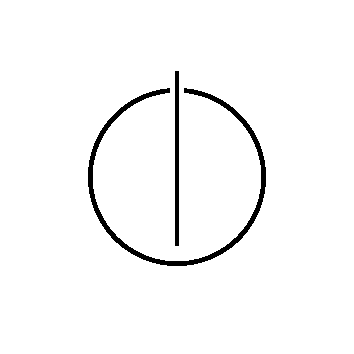
\includegraphics[width=4cm]{styles/informat.png}
  \end{figure}
  
  \end{center}

	\clearemptydoublepage
	
	% The titlepage for the CAMP report document.
% Included by MAIN.TEX


%--------------------------------------------------
% The title page
%--------------------------------------------------

% correct BCOR - undo at the end !!!
\def\bcorcor{0.15cm}
\addtolength{\hoffset}{\bcorcor}

\thispagestyle{empty}

\vspace{10mm}
\begin{center}
	       \oTUM{4cm}
	   
	   \vspace{5mm}     
	   \huge FAKULT{\"A}T F{\"U}R INFORMATIK\\ 
	   \vspace{0.5cm}
	 \large DER TECHNISCHEN UNIVERSIT{\"A}T M{\"U}NCHEN\\        
	 
\end{center}


\vspace{5mm}
\begin{center}

   {\Large \doctype}

  \vspace{5mm}
  
  {\Large \title}\\
  
  
  \vspace{5mm}
  
  
  {\Large  \titleGer}\\
  
  
  \vspace{10mm}

   % \hfill
    \begin{tabular}{ll}
	   \large Author:	& \large \author \\[2mm]
	   \large Supervisor:	& \large Prof. Dr. rer. pol. Hans-Arno Jacobsen  \\[2mm]				
	   \large Advisor:	& \large \begin{minipage}[t]{1.0\columnwidth}
		 Martin Jergler, M.Sc.
	     \end{minipage} \\[10mm]
	     
	   \large Date:	& \large November 15, 2016
	 \end{tabular}
	 
	 \vspace{5mm}
	 
	 \begin{figure}[H]
  \centering
   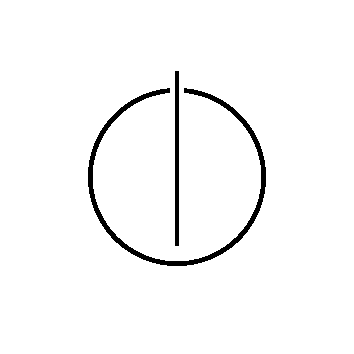
\includegraphics[width=4cm]{styles/informat.png}
  \end{figure}
   

\end{center}

% undo BCOR correction
\addtolength{\hoffset}{\bcorcor}
	
	\clearemptydoublepage


\thispagestyle{empty}
\selectlanguage{german}
	\vspace*{0.6\textheight}
	\noindent
	Ich versichere, dass ich diese Bachelor-Thesis selbst{\"a}ndig verfasst und nur 
	die angegebenen Quellen und Hilfsmittel verwendet habe.
	
	\vspace{20mm}
	
	\selectlanguage{english}
	\noindent
	I confirm that this bachelor's thesis is my own work and I have documented all sources and 		material used.
	
	\vspace{10mm}
	\noindent
	Munich, November 15, 2016 \hspace{4cm} \author
	\selectlanguage{english}
\newpage
	
	% Abstract for the TUM report document
% Included by MAIN.TEX

\clearemptydoublepage
\phantomsection
\addcontentsline{toc}{chapter}{Abstract}	

\vspace*{2cm}
\begin{center}
{\Large \bf Abstract}
\end{center}
	
	\clearemptydoublepage
\phantomsection
\addcontentsline{toc}{chapter}{Acknowledgements}	


%\chapter*{Acknowledgements}

\vspace*{2cm}

\begin{center}
{\Large \bf Acknowledgments}
\end{center}

\vspace{1cm}


	
	\clearemptydoublepage
\phantomsection
\addcontentsline{toc}{chapter}{Acronyms}	



%\chapter*{Acknowledgements}

\vspace*{2cm}

\begin{center}
{\Large \bf Acronyms}
\end{center}
\vspace{1cm}

\begin{acronym}[bash]
\acro{CMMN} {Case Management and Notation Model}
\acro {DMN} {Decision Model and Notation}
\acro {OMG} {Object Management Group}
\acro {BPMN} {Business Process Model and Notation}
\acro {BPM} {Business Process Management}
\acro {ARIS} {Architecture of Integrated Information Systems}
\acro {BPR} {Business Process Redesign} 
\acro {IBM} {International Business Machines Corporation}
\acro {BPMI} {Business Process Management Initiative}
\acro {BPEL} {Business Process Execution Language}
\acro {UML} {Unified Modeling Language}
\acro {DRD} {Decision Requirement Diagram}
\acro {CM} {Case Management}
\acro {ACM} {Adaptive Case Management}
\acro {DRG} {Decision Requirement Graph}
\acro {FEEL} {Friendly Enough Expression Language}
\acro {SQL} {Structured Query Language}
\acro {PMML} {Predictive Model Markup Language}
\end{acronym}


	\clearemptydoublepage
	\phantomsection
	\addcontentsline{toc}{chapter}{Table of contents}
	\tableofcontents
  	\clearemptydoublepage
  
	\mainmatter
		% Included by MAIN.TEX
% Put your content in here or include it by using \input (\include won't work)

\addtolength{\evensidemargin}{-12mm}

% ---------------------------------------------------------------------------
%
%Introduction and Background Theory
%
% ---------------------------------------------------------------------------
\part[Introduction]{Introduction}
\label{part:introAndBackgroundTheory}
\chapter{Introduction}
\label{chapter:introduction}

\section{Motivation}
\label{chapter:motivation}
Since its beginning in the early 1980s, Business Process Management (BPM) has become a large industry and research field. Starting with Business Process Re-engineering (BPR), a radical approach to align internal business processes along the value chain of a company, many subsequent modeling techniques were developed. \\
With the release of Business Process Model and Notation (BPMN) in the early 2000s, a step towards automated process execution has been taken. Since the initial release, BPMN has been examined thoroughly which lead to several positive and negative conclusions. The lack of flexibility for processes that rather require knowledge instead of a strict control flow, only to mention one. For this reason, Case Management Model and Notation (CMMN) was published in 2014. A modeling notation capturing flexible work with focus on knowledge workers and support for run-time adjustment such as planning and skipping tasks, or even adding new ones. \\
Another modeling specification was released in 2015 by the Object Management Group (OMG): the Decision Model and Notation. Where BPMN gets stuck with its vast amount of gateways capturing decisions, DMN becomes relevant by reducing decisions to a single element, the Decision Table. \\
All of the three named modeling techniques contribute to the objective of fully automated process execution and the reduction of routine work. Furthermore, processing data and supporting knowledge-intensive jobs moved to the center of current process modeling and ongoing research. \enlargethispage{1\baselineskip} \newpage

\section{Problem Statement}
\label{chapter:problem_statement}
Business Model and Notation (BPMN) has become a quasi-standard for modeling business processes, logical steps in software-systems or for the alignment of companies along the process chains. BPMN was standardized in 2005 by the Object Management Group (OMG), but had a long list of predecessors including the \textit{Event-driven Process Chain} (EPC), the \textit{Swimlane Visualization}, \textit{Business Process Re-engineering}, to mention only a few. Despite the inheritance of these languages, BPMN is not a fit for all solution. It has positive and negative aspects, which will be discussed in this thesis.\\ 
BPMN works best when it comes to processes that incorporate the \textit{Value Chain Model} by Michael E. Porter \cite{Porter1988}. Every company needs these strict processes to optimize the value chain, for the value creation and to separate the hierarchies between employees and departments. By 2016, however, these processes have been largely automated. For this automation, the BPMN syntax worked very well due to the strict processes that could be automated more or less easily. The next challenge is to implement a process that can help manual workers and deal with data intensive environments. \\
At this point, \textit{Case Management Model and Notation} (CMMN) and \textit{Decision Model and Notation} (DMN) come into play. Both were highly anticipated by people working in modeling departments. This thesis will investigate the benefits of separating the decision logic and case management into these new standards, as well as combining them in a macro model. The weaknesses and strengthens of BPMN, CMMN and DMN will be presented in detail in order to form indicators for when to use which language best. The publication of the two latest standards by the Object Management Group lead to the following research tasks: 

\begin{itemize}
\item Investigation of the new Decision Model and Notation specification published by the Object Management Group, extracting the assets and drawbacks especially concerning the vast modeling of gateways in BPMN. Is DMN the solution to simplify decision-modeling? 
\item Investigation of the Case Management Model and Notation specification by the Object Management Group, particularly how case modeling can be used in a model-driven software development project. 
\item How do CMMN, DMN and BPMN work together in a model-driven software project? Is there a valid possibility to combine all three specifications in one model? Is it possible to improve the process and information flow, readability and eventually implementation of the model by the developer? \enlargethispage{1\baselineskip}  
\end{itemize}

\section{Approach}
\label{chapter:approach}
The intent is to create a guideline for differentiating and combining three modeling languages. The main topics covered are an explanation of the specifications, the main characteristics, a set of tools that identifies each notation and eventually a practical application to show how the guideline works. \\
At first, a background section derived from literature analysis gives an overview of each specification's development up to the recent release of standardization. Followed by a set of process discovery methods derived from a literature review, the reader is instructed on how to aggregate information about processes. Furthermore, the different methodologies are listed with positive and negative aspects, as well as some best practices derived from conference publications. \\
Afterwards, each notation is explained with illustrations, focused on the main characteristics. With the help of the specifications and additional literature, a set of categories and specific terms was constructed aiming at the correct identification of a notation for a given process discovery output. As a consequence, the modeler is able to discover processes and differentiate between the notations. \\
Next, the specifications are examined for technical interfaces to different modeling notations. Along with practical examples, the attributes and references to different notations are shown. Moreover, this part deals with best practices and patterns used to combine different notations. \\
The third chapter is comprised of a practical application to processes taken from the eKultur GmbH. eKultur, as described more detailed in the background chapter, is a software project to digitize the theater production industry. The company has chosen a model-driven development approach with the side effect of generating several process models. After the process discovery phase, the results were used to apply the indicators and check the recommendation system, as well as modeling the processes. A decision-engine was designed to simplify the application of indicators and is presented as well in Chapter \ref{chapter:case_study}. \\
Each model featured in this thesis was created with either \textit{signavio modeler} or \textit{camunda modeler}, relating to either a specific process taken from eKultur GmbH or a certain use case which has an explanation next to it. \newpage

\section{Contributions}
\label{chapter:contributions}
Since the release of CMMN in 2014 and DMN in 2015, recent publications deal with their realization in platforms and the proof of concept, e.g. \cite{KurzSchmidtFleischmannEtAl2015}, \cite{Fish2012}, \cite{OsuszekStanek2015}. Recent publications deal with Case Management or Decision Management on a higher level concept while former publications incorporate a broader research field influencing the notation as well. \\
None of the publications, however, deal with the combination of all three modeling languages or the objective to take process discovery results and examine them for a fitting modeling notation. This thesis contributes to the BPM research field in two ways: as a summary of the current state of these three notations and best practices, as well as a methodology to identify a suitable notation for a given process documentation. 

\section{Organization}
\label{chapter:organization}
Before the actual analysis and creation of the guideline commences in Chapter \ref{chapter:indicators}, Chapter \ref{chapter:background} illustrates the development of the each specification's origins up to the current state. To understand the usage and necessity for each specification, it is important to understand what researchers and people from the corresponding industries motivated to develop a new modeling language. \\
The background part is followed by the compilation of indicators. Each modeling language has a certain domain where it works best. The intent of this thesis is to serve as a guideline to differentiate between and combine the three named modeling languages. As a consequence, the indicators will help analysts with the decision-making process and identify the appropriate modeling language for a given process. \\
In Chapter \ref{chapter:combination}, each specification is examined for interfaces to different modeling techniques, followed by the case study that shows a practical application of the indicators on process models taken from eKultur GmbH. This part also deals with the results found in the case study. \\
In the last chapter, we discuss the indicators and the case study, as well as positive and negative aspects of this thesis. Furthermore, recommendations for future work are provided.

%\part[Preliminaries]{Preliminaries}
%\label{part:preliminaries}
%\chapter{Preliminaries}
\label{chapter:preliminaries}

\part[Related Work]{Related Work}
\label{part:relatedWork}
\chapter{Related Work}
\label{chapter:related work}

\section{BPMN}
 -- todo 
 
 Geplant: Am Ende der Ausarbeitung 
 
 
\section{CMMN}
Case Management and knowledge work are not brand new inventions that have been created in the past few years. "Peter F. Drucker made the first reference to knowledge work in (...) 1959 (...)" \cite{Motahari-NezhadSwenson2013}. A current "overview and research challenges" provide \cite{Motahari-NezhadSwenson2013} who explain the difference between business process management and adaptive case management. They briefly sum up the state of the art in case management technology and the next generation solutions. 
Mentioning technology and tools for Case Management, CMMN and Adaptive Case Management, there are many articles dealing with these topics. \cite{OsuszekStanek2015} describe how adaptive case management can be implemented in businesses and integrated in Enterprise Resource Planing systems (ERP). Additionally they approach a new architecture which decouples decision logic, knowledge work and process flows. All this leads to a better handling of information and an optimization of business modeling. 
Another practical example provide \cite{Kuzin2013} explaining the company's approach towards an implementation of the CMMN paradigm. This includes the ability to change requirements or orders during run-time, which is one of the major aspects in their system. To achieve this goal, they first set up a meta model of their order-based system and enhanced it afterwards. 
These practical examples are important in order to evaluate the compatibility with the CMMN specification and other modeling languages, specifically BPMN. They also provide a good overview of how to combine modeling techniques and how they are realized as a system in companies. 
A more theoretical approach to case management and CMMN particularly provide \cite{WangTraore2014} and \cite{Zeising_2014}. They both do research on transforming CMMN into different languages. \cite{WangTraore2014} do model-to-model transformation from CMMN to  DDML (DEVS-driven Modeling Language) which is used to formalize CMMN and analyze it afterwards. \cite{Zeising_2014} have a similar approach, but a different goal. Due to weaknesses of CMMN, the language cannot be used to create a platform for both agile and route processes. They describe agile processes as the ones "(...) of which the exact flow cannot be determined completely a priori" \cite{Zeising_2014}, which is a fundamental characteristic of knowledge work and the reason why case management is so important for many industries. Coping with CMMN's downsides they build their platform on a "rule-based cross-perspective and model intermediate language on textual basis, (...) called \textit{Declarative Process Intermediate Language (DPIL)}" \cite{Zeising_2014}. \\
A useful source for evaluating CMMN as a standardization for adaptive case management is \cite{KurzSchmidtFleischmannEtAl2015}. The subtitle \textit{Examining the applicability of a new OMG standard for adaptive case management} is a good foundation to see how OMG met the expectations from the industry and researchers. This paper sets up requirements deriving from different sources described in detail in section two \cite{KurzSchmidtFleischmannEtAl2015}. At the end of their paper, they evaluate how good the requirements were fulfilled by the CMMN standardization and provide feedback for future improvements. 

\section{DMN}
The Decision Model and Notation standardization was meant to improve the \textit{separation of concerns} \cite{BiardMauffBigandEtAl2015} which is the decoupling of decision logic and the control-flow. Biard et al. investigate how the new standard DMN can be used for decoupling BPMN and the decisions modeled as gateways. Decision-modeling is not typically included in control-flow oriented modeling languages. BPMN has not the power to model vast decision-trees due to the gateway restrictions. \cite{BatoulisMeyerBazhenovaEtAl2015} even calls it a "(...) [misuse] for modeling decision logic". They found an autonomous way of separating the concerns. After averaging more than 900 models from different industries they introduced a "(...) semi-automatic approach to identify decision logic in business processes (...)" \cite{BatoulisMeyerBazhenovaEtAl2015}. This semi-automatic approach incorporates the 900+ models they used to identify patterns in decision modeling. Formalization is not one of the key issues in this thesis, but the translation of BPMN to DMN or the link between them definitely is. 
Evaluating the compatibility of DMN with different modeling languages has been the objective of \cite{MertensGaillyPoels2015}. They approached a combined solution for knowledge-intensive work modeling and extracting the decision logic, what lead them to a new language called \textit{Declare-R-DMN}. Although the Declare language is not part of this thesis, the combination of it with DMN is useful to evaluate the compatibility with BPMN and CMMN. 

\part[Background]{Background}
\label{part:background}
\chapter{The Evolution from BPMN to CMMN and DMN }
\label{chapter:Background}

\section{BPMN and its shortcomings}
\subsection{Origins of BPMN}
The evolution of business processes and process thinking dates back to the 1980s when Michael Porter developed the \textit{Value Chain} making a first proposal on how to align companies along the business processes \cite{Porter1988}. 
This major step initiated consecutive research and improvements in the field of business process engineering and re-engineering. The latter has been a very popular technique for companies to strip down their legacy processes, optimize them and implement the new ones. A very prominent example is Ford who copied the Mazda's concept of a central database replacing an old fashioned paper stream \cite{Dumas2013}. \\
Inspired by Ford and Mazda, the \textit{Business Process Redesign} (BPR) was emerging in until the late 1990s. At that time, companies tried to redesign in a radical manner the way processes, people and data keeping works. Dumas et al. define four reasons for the fall of BPR, whereof over-radicalism might be the most influential one \cite{Dumas2013}. \\

Despite the fall of BPR, the management of business processes became a prominent part of business optimization. Consequential different methodologies like the \textit{BPM lifecycle} or the \textit{Architecture of Integrated Information Systems} (ARIS) were born along with new modeling languages. "ARIS [also] provides a modeling language known as event-driven process chains (EPCs)" \cite{Lankhorst2009}. By today, ARIS still is a very popular, thus a well known, methodology for enterprise modeling and EPCs a widely used modeling language for event-driven processes, as the name states. \\
ARIS was published 1994 by August Wilhelm Scheer, a researcher for Business Information Systems at the Saarland University. Around ten years later, Stephen A. White and the \textit{Business Process Management Initiative}, consisting of roughly 35 individuals and companies total, published the first version of the new \textit{Business Process Modeling and Notation} (BPMN) concept \cite{Allweyer2010}. In 2006, the OMG adopted BPMN as well as the BPMI and published an overhauled version, BPMN v. 2.0 in 2011. This version was highly anticipated and had to meet high expectations. The goal was to create a language with the ability to interchange modeling tools. New parts were added such as the \textit{Choreography diagram} for modeling data exchange between partners and the \textit{Conversation diagram} showing the relationship between several partners \cite{Allweyer2010}. 

\subsection{Shortcomings} 
"As the name already indicates, BPMN is restricted to process modeling [...]" \cite{Lankhorst2009}. The goal in terms of BPMN was to create a powerful tool for modeling traditional processes. BPMN is an interchangeable language predestined as a middleware between the database and software layers. It has the ability to be executed \textit{Business Process Execution Language} (BPEL) and a well-known set of symbols and artifacts for modeling the diagrams. Additionally, it inherited its simplicity from EPCs and the \textit{Unified Modeling Language} (UML), which is also part of the OMG family. \\
This simplicity, however, has limitations when it comes to agile and decision intensive models. Decisions, for instance, are illustrated by gateways. These gateways work as connectors separating the process flow into different branches. Each branch has a token wandering in flow direction through the graph. But what if a business wants to change decisions in real time without losing the tokens flowing through the chart? At the current state of development, which is BPMN v 2.0.2, there is no possibility to do so. This is only one of the problems which \cite{Repa2014} and \cite{ReckerIndulskaRosemannEtAl2006} investigated more closely. They both came to the conclusion that BPMN is lacking the ability implement business rules which leads the user to display them in spreadsheets. 
Another downside is the impossibility of modeling agile processes. People working in departments which do not have strict processes but more agile ones cannot use the supportive power of BPMN or process optimization. Despite their knowledge intensive work, they still can benefit from optimizing workflows, or even help new employees getting known to their new job in the department. In this thesis, we will not focus on \ac{BPMN}'s syntax deficits but more on the possibility CMMN and DMN offer. 

\section{Origins of CMMN}
\ac{CMMN} was standardized by the \ac{OMG} in 2014 which represented a peak in terms of notation for the case management research. However, research began more than ten years ago when Wil Van der Aalst first published his paper about case handling offering a new approach for flexible processes \cite{aalst2003}. He summarized different opinions from several authors into the statement that contemporary workflow-systems were not able to handle flexible processes. To be precise, he identified four problems: 
\begin{itemize}
\item work needs to be divided into atomic steps, so called 
\item the routing of activities was used to distribute the tasks and authorize workers the workers to do them 
\item \textit{context tunneling}: workers only focused on the process flow but not on the context surrounding the activities
\item the individual's focus was more on what \textit{should} be done instead of what \textit{cane} be done 
\end{itemize} 

He portrayed a \textit{blind surgeon} as a metaphor who incorporates the four problems in his daily work, for instance refusing a blood sample when it was necessary but not part of the problem in case of what could be done and what should be done \cite{aalst2003}.
Consequently he solved the problems inventing an adapted model for cases, which consists of objects that can be found in the OMG'S specification from 2014 as well. In \ref{tab:casehandling} a comparison of the key objects of Case Handling and CMMN is provided. The Case Handling's key objects are:
\begin{itemize}
\item activities or tasks which are the atomic unit of work
\item Actors with roles who execute, skip or redo the tasks
\item Case representing the product the actor is producing 
\item data objects for information and values 
\item forms that present data objects from different point of views 
\end{itemize}
% Please add the following required packages to your document preamble:
% \usepackage{booktabs}
% \usepackage{graphicx}
\begin{table}[]
\centering
\caption{Comparison CMMN and Case Handling Model}
\label{tab:casehandling}
\resizebox{\textwidth}{!}{%
\begin{tabular}{@{}lll@{}}
\toprule
                           & van der Aalst    & CMMN Specification        \\ \midrule
Product                    & Case             & Case                      \\ \midrule
Atomic Unit of work        & Activity / Task  & Task                      \\ \midrule
Information Handler        & Data Object      & Case File Items           \\ \midrule
Information Representation & Forms            &                           \\ \midrule
Executing Person           & Actors and Roles & Human tasks with asignees \\ \midrule
Connectors                 & not specified    & specified                 \\ \midrule
Triggers                   & not specified    & Event Listeners           \\ \bottomrule
\end{tabular}%
}
\end{table}

Van der Aalst proved his concept practically in a joint venture with dutch Construction company. They applied the Case Handling model and built a prototype with FLOWer resulting in a rudimentary worklfow management system. They requested workers to use the system during their work and evaluated the prototype in the end. Van der Aalst calculated a Return on Investment (ROI) of 0.7 to 1.4 years in the year 2002 \cite{aalst2003}. With today's workflow management systems, the ROI would presumably be much higher. 

\section{Origins of DMN}
The \acl{DMN} language describes processes in a different way as \ac{BPMN} does. They differ in their way of how to achieve the actual goal of the process. BPMN, for instance, describes an imperative way. Goedertiert et al. define imperative as "[...] [focusing] on providing a precise definition of the control-flow of the business process in a graph-based process modeling language" \cite{Goedertier2013}. In order to model decisions, BPMN has a rich amount of gateways to direct the control-flow into the desired tasks depending on the decisions being made. Additionally BPMN provides a Business Rule Task sending data to and receiving it from a business rule engine \cite{BPMNspec}. However, this business rule task " [...] cannot be decomposed any further - and involves no user interaction" \cite{Fish2012}. Thus the modeler is not able to define roles for decision, define any requirements for these and is not able to decompose them into fine-grained steps. This might be unnecessary for simple decisions, but in larger and more sophisticated diagrams, complex decisions cause huge branches in the control-flow making the diagram confusing the reader. \cite{MendlingReijersAalst2010} formulated \textit{Seven Process Modeling Guidelines} according to an empirical study. They built an EPC model with various branches connected by \textit{AND}, \textit{OR} and \textit{XOR} connections. Additionally they violated naming conventions and used multiple end points. One of the resulting guidelines (G1) states "Use as few elements in the model as possible" \cite{MendlingReijersAalst2010}, which is contradicting the imperative way of modeling decisions in BPMN.  
In this situation, declarative modeling approaches are more appropriate. According to Alan Fish, declarative languages "[...] focus on what should be done in order to achieve business goals, without prescribing how an end state should be reached" \cite{Fish2012}. The CMMN specification is a declarative modeling approach as well, whereas EPCs and BPMN aren't. 
Fish also described a way to refine the decision requirements. He invented the \ac{DRD} to show " [...] the structure of the required decision-making as a network of decisions and subdecisions with their supporting areas of business knowledge and data" \cite{Fish2012}. The main use for this DRD is to make knowledge involved in decision-making explicit instead of implicit. 
In the \ac{DMN} Specification by the Object Management Group, a DRD can also be found. This DRD includes the elements as Fish invented for his DRD: Decisions, Input Data (Fish: Data area), Knowledge Source (Fish: Knowledge Area). However, the OMG's DRD is a much more refined modeling approach since it incorporates Fish's DRD and is under constant development. 
Summarizing the findings, the DMN technique is derived from Fish's findings on how to automate decisions and the declarative modeling approaches which supplement BPMN with tools to model processes without strict control-flows.  

\part{Indicators}
\label{part:indicators}
\chapter{Differentiating between BPMN, CMMN and DMN}
\label{chapter:indicators}

Starting with process management for some companies means for many companies to build up their infrastructure, workflows and eventually models on a greenfield. The following sections provide a brief overview of process discovery techniques (manually as well as automated). It starts with data sources and ends with process maps. Building on process maps and the associated documentation, indicators for the differentiation between BPMN, CMMN and DMN are introduced. Terms and categories will be explained as well as the derivation of each set of indicators along with an explanation of the associated standard. 

\section{Discovering the processes}
\label{section:process_discovery}
% Diesen satz kann man gerne woanders wiederverwenden ---- Some researches like Van der Aalst et al. \cite{Aalst2011} put process mining and process discovery on the same semantical level, wherefore different researchers like Laury Verner \cite{Verner2004} don't. 
Processes are resources. Similar to iron or copper, processes are deeply embedded in the bedrock of a company and need to be discovered. This metaphor is not even far-fetched, since the correct terms for gathering information is \textit{process mining} or \textit{process discovery}.
In this chapter, the aggregation of information before the actual process modeling will be discussed, specifically two approaches: A manual one (often referred to as process discovery) and an automated one (often referred to as process mining). Both techniques will be discussed briefly and put in the context of the eKulturPortal venture. 

\subsection{The manual way}
According to the BPM Lifecycle \cite{Dumas2013}, gathering information begins with identifying the process. This first leads to the accumulation of all the relevant processes sorrounding an initial question like \textit{How does the process work at the moment?} or \textit{What / Who contributes to this process?} \cite{Dumas2013}. Ideally, the accumulation shows the posed question in a map surrounded by all the relevant processes. The way this map is created is up to the involved personnel. It can very from a mind-map to a more detailed flowchart or even something similar to a BPMN or EPC diagram. In the end, this map is useful for process discovery. \\
Laury Verner identified three "key players" \cite{Verner2004} in the process discovery phase: 
\begin{itemize}
\item "The Sponsor", who decides the scope and the goal that needs to be achieved and is also called the \textit{Process Owner}.
\item "The Subject Matter Expert" (SME) who is also referred to as the \textit{Domain Expert} since he is the person working with the processes.
\item "The Analyst", often referred to as \textit{Business Analyst}, who is the expert for modeling and designing the processes. 
\end{itemize}

These three roles are commonly assigned to various people in large companies. To begin with process discovery, the process owner sets the goal such as optimizing a department's workflow or integrating automation into manual processes. He is the one who is responsible for the whole project and has to monitor the progress. \\
The SME or domain expert is the employee executing the process. SMEs are the subject of every process discovery technique due to their role as knowledge source. A process analyst has to extract the knowledge they implicitly keep and to visualize it as explicit processes. The one created are most commonly not the ones which are presented as results. However, it is important for the progress of such a project to visualize the gathered knowledge. \\
The following process discovery techniques are summarized by Marlon Dumas et al. in \cite{Dumas2013} in a theoretic way, which are emphasized by \cite{Verner2004} and \cite{Jadhav2011}. \\
Dumas categorizes three different approaches in terms of process discovery: The "evidence-based discovery", the "interview-based discovery" and the "workshop-based discovery" \cite{Dumas2013}. Each approach deals with different input sources. \\
The \textbf{evidence-based discovery,} deals with documents, models, observations and event logs\footnote{Dumas et al. include event logs in his manual approach for the reason of integrity}. The process analyst may choose different approaches in the evidence-based category: He may either examine the documents and aggregate the information which can be found there; he may also choose to observe the employee by playing an active part in the process or just passively watching the employee work; or he may work with the event logs according to \cite{Dumas2013}, which will be explained in the automatic section in more detail. \\
Each decision bears several advantages and challenges that need to be kept in mind: \\


\textit{Advantages:}
\begin{itemize}
\item Choosing the document analysis, an analyst can identify workflows in the company and the cooperation of different departments. He gets an overview of how the company works and can understand the as-is process better \cite{Dumas2013}. 
\item Documentation provides an unbiased view of the processes, if it is not written by a single person. 
\item Observation is good to get a detailed understanding of how a process works. The analyst observes the SME by initiating either an active instance of a process (e.g. ordering a product as a customer) or by playing a passive role and just observing how the employee works \cite{Dumas2013}. 
\item Observation additionally shows the boundaries, milestones and interfaces to different processes.
\end{itemize}

\textit{Challenges:}
\begin{itemize}
\item Documentation is not written process-ready, so the analyst needs to aggregate the information to fit the process. 
\item The work described in documentation might not fit the granularity level of the process \cite{Dumas2013}. Often the step by step documentation is either too detailed or does only cover a high level view without necessary details about interfaces to different processes. 
\item The biggest challenge regarding the documentation is to keep it up to date. While the system is developing, in some cases the documentation has been written initially but never been updated. 
\item Observation might lead to wrong results because employees work different when they are observed. They might want to show the best practice example and leave out occurring failures. 
\item Observing an employee might only show one perspective of the process but not different ones such as the customer perspective. In this case, the analyst is intended to switch between the passive and active roles to get a thorough overview. 
\end{itemize}

The \textbf{interview-based strategy} works in a different way: The analyst sets up an interview with a domain expert. In this case, there is no specific input data involved except from the knowledge the domain expert has. Dumas et al. provide two paths the interviewer can guide the SME through the interrogation: backwards (from the product to the start) or forwards (start to product). Each direction has advantages: Backwards shows the input data the process has to wait for, whereas forwards clarifies the path of the process and how the employee works \cite{Dumas2013}. Interview-based discovery has the following advantages and challenges: \\

\textit{Advantages:}
\begin{itemize}
\item The person directly involved can explain the process in detail, which results in a current view of the processes with advantages and downsides directly from the workers. Later, the process design benefits from this additional information.
\item Different routes show the process from various angles. "This is particularly helpful for understanding which decisions are taken at a given state" \cite{Dumas2013}.
\item By interviewing various employees, a centralized documentation of the knowledge can be created that might not have been existing before.
\end{itemize}

\textit{Challenges:}
\begin{itemize}
\item Interviews require proper planning: Each process activity needs to be clarified, the expected outcome of the process needs to be defined, all the necessary input data from interface processes has to be clarified and all the subsequent processes need to be mentioned. 
\item The analyst may need various iterations. Each interview leads to a script that needs to be transformed into a model, which then has to be verified by the interviewee again.
\item Structured vs. free-from interviews: In the free-form interview, SMEs are completely "uncensored" \cite{Verner2004} and free to mention everything they associate with the process. In structured interviews, workers answer to "pre-defined questions" \cite{Verner2004}. The former method captures a larger picture of the process, the latter one provides a better understanding and more details for the analyst. 
\item Similar to the evidence-based method, the interviewee might hide or not mention failures which are necessary to be discovered by the analyst.
\end{itemize}

A third method is the \textbf{workshop-based discovery}. Unlike in interviews, workshops include a group of SMEs, several analysts and one or more process owners. In these situations it is eminent to have a \textit{facilitator} who is responsible for the "verbal contributions" \cite{Dumas2013}. A recommended practice is to create the models directly during the workshops. The resulting illustrations are not the desired output, but it is possible to create a process map or brief processes that can be revised in future iterations. Dumas calls the responsible person the \textit{tool operator} \cite{Dumas2013}. \\

\textit{Advantages:}
\begin{itemize}
\item A workshop combines different views on a process at once and offers the possibility to create a rich and detailed model through several iterations \cite{Dumas2013}. 
\item Models can be created simultaneously. 
\item Involved analysts have the same level of knowledge, thus have an advantage in the design stadium.
\end{itemize}

\textit{Challenges:}
\begin{itemize}
\item Workshops need several iterations and are very similar to meetings. Each meeting needs preparation, a minute keeper and someone taking notes. In this case, the facilitator and the tool operator need to be well prepared to facilitate the expected outcome with the participants.
\item The attendance of process owners may influence the employees, consequently they might not talk about failures or downsides of involved steps. 
\item The anticipated level of detail needs to be defined before the meeting starts to differentiate between unnecessary tasks, like "putting the document on a fax machine" \cite{Dumas2013}, and the ones essential for the model. 
\item Workshops are very time consuming and need to be planned in advance to cover all the roles in the workshop.
\end{itemize}

Apart from the three described methodologies, their challenges and advantages, there are a few meta-questions that need to be answered according to \cite{Verner2004}:
\begin{itemize}
\item Centralized vs. distributed approach: The analyst needs to decide whether workshops or interviews work best in the specific situation.
\item Top-down vs. bottom-up: Is it better to start from the top (e.g. the output of each process) and proceed until the smallest tasks are reached, or is it better to start from the bottom (the smallest tasks) and aggregate the model from the bottom up? 
\item Free vs. structured form: As mentioned in the interview-based strategy, a workshop or interview can be held in a free from way or in a structured one. 
\end{itemize}

Verner \cite{Verner2004} also offers a recommendation that is also used in the eKulturPortal context: 
\begin{enumerate}
\item "Start with a top-down view of the processes. Cluster the processes in a map for navigation purposes and get an overview of how the company works. This can be done by interviews and documentation analysis."
\item "Use bottom-up structured interviews to clarify the details and use the created map to validate them. The resulting outcome is an as-is process model that needs to be verified in step three."
\item "Create integrated models of the processes and validate them with stakeholders such as process owners in a workshop. These models are a good base for discussions and lead to structured outcomes." 
\end{enumerate}

Each scenario needs its own approach. However, the recommendation from Laury Verner worked for the eKulturPortal venture in a highly unstructured context. Here, knowledge is implicit and a mix of documentation analysis, interviews and workshops were necessary. Although adapting the mix, the actual structure of the recommendation was maintained. In the eKulturPortal context, there hasn't been any as-is documentation but SMEs that were observed and interviewed in a free-form way. Additionally, workshops were mostly inefficient due to the missing facilitator and tool operator. The involved domain experts had dual roles combining an SME and a process owner. This made it complicated to differentiate between process knowledge and goals that need to be achieved. 
The outcome was a combined approach of observation and interviewing simultaneously. 

\subsection{The automated way}
Small companies or such without any supporting IT infrastructure might rely on the manual way of process discovery. However, there is an option for automation: the \textit{automated process discovery} (ADP) \cite{Dumas2013}. This method uses event logs of a workflow management system. ADP is a sub-category of the \textit{Process mining} research field, which will be discussed briefly in this section.\\
The term process mining originates from the very similar technique called \textit{Data mining}. Both approaches use a set of input data to transform it into a desired output structure like a spreadsheet, trees or rules, cluster etc. \cite{Aalst2011}. Process mining combines three different strategies: the process \textit{discovery}, \textit{conformance} and \textit{enhancement}. The first phase is corresponding to the preceding section: The system uses event logs to create models that have been unknown or implicit before. This phase works without any pre-defined input data apart from the logs. \\
Conformance takes an existing process and the corresponding event logs to compare them. The goal of this comparison is to check whether the model matches the executed process and vice versa \cite{Aalst2011}. 
In the enhancement phase, the process generated from the event logs \textit{enhances} the pre-defined models. The desired result is a model that matches the real executed process by either repairing the models or extend them with another perspective \cite{Aalst2011}. 
Depending on the infrastructure the executing company uses, it is up to their discretion about the phase to start with. For the purpose of this thesis, we start with the discovery phase and assume there are no a priori models given. \\
The very first requirement for process mining is the conformance of event logs. Scanning data storage for event logs often results in various outputs. They might be scattered across departments, stored in various formats and - most importantly - not prepared for process mining. Solving this problem needs a three-way paradigm: \textit{extract, transform and load} \cite{Aalst2011}. At first, the data needs to be extracted from the data storage and aggregated in a central warehouse for the process mining. Next, the data needs to be transformed to meet the requirements. This means, the event logs need to have at least an identification for the corresponding process and an activity column \cite{Aalst2011}. With these two columns, the events occurring in the log can be ordered and the model can be generated accordingly. Without either ordering or activities, there is no possibility to create a model. \\
Third, the transformed tableau is loaded into the target system where process mining takes place. The more data is included in the logs, the more useful the output is for the later conformance and enhancement phase. Helpful additions are costs of paths and timestamps. With these two extra columns it is possible to analyze the critical path with e.g. the \textit{Critical Path Method} (CPM) \cite{Domschke2015}. Timestamps solve another problem of event logs: Imagine two instances of the same activity start at different times. Which one is the first that stops and which one the last?\enlargethispage{1\baselineskip} \cite{Aalst2011} illustrates this example for event logs with an insufficient amount of attributes. \\
After the event logs are transformed and loaded into the target system, the analysts need to decide how to cluster the data. A well-known example is the \textalpha -algorithm invented and described by \cite{Aalst2011}. This algorithm takes an event log and creates a \textit{WF-net}, which are "[...] a natural subclass of Petri nets tailored towards the modeling and analysis of operational processes" \cite{Aalst2011}. Apart form this theoretic approach, tools like ProM\footnote{for further information see \url{http://www.promtools.org/doku.php} (Sept. 12, 2016)} offer plugins with algorithms that can be selected according to the desired input and output. An example is the Mutli-phase miner that generates and EPC from the causal dependencies in the event log \cite{Weimer2006}. This makes it easy for practical uses of the process mining approach and leads to fast results compared to the manual method. \\
Each of the mentioned phases (discovery, conformance, enhancement) are optional and it is to the analyst's discretion what has to be executed. However, the discovery does not improve the as-is state, it only describes it. It is recommended to do each phase of the process mining to get the desired results and to check, if the implemented processes achieve the intention designed in the models. \\
The process mining advantages are: 
\begin{itemize}
\item Accurate results describing the real-time status of the process. 
\item Fast method that can be tracked in real-time. 
\item Real-time monitoring of processes in a map-like structure. 
\end{itemize} 
 
And the challenges according to \cite{manifesto2011} and \cite{Dumas2013} are:
\begin{itemize}
\item Aggregating the data in a format the process mining tool can handle and the output requires. 
\item Understanding the resulting models, as they can be very complex and hard to read for the analysts.
\item Asking the right questions: Taken into account that companies use ERP-systems with sometimes more than 10,000 data points, it is necessary to define the right question and extract the right data. 
\item Dealing with bias and noise resulting from vast amounts of data. 
\end{itemize}

Both, the process mining and manual process discovery strategies provide methodologies that lead to the desired as-is and to-be models. It is up to the skills of the analysts, to the IT infrastructure of the company and the objective set for the whole project to choose which method is being used. 

\section{Introducing the indicators}
\label{section:indicator_introduction}
In the preceding section, two major approaches on how to aggregate input data were explained: the manual process discovery as a set of tools to get information from SMEs or process owners, the automated process discovery (or process mining) as a methodology to scan event logs of workflow management systems and generate models according to algorithms. Both techniques result in process maps and / or documentation, e.g. spreadsheets, textual descriptions and interview transcripts. The next step is to choose the correct modeling language to either do an as-is model or start with the design model. Most commonly, an as-is model is built as the foundation for further analysis, followed by the to-be model. \\
In this section, the conduction of indicators will be introduced and explained. Indicators, in general, are tools that take an input and present the user a value or a choice that should be made. The subsequent indicators are intended to help the analyst to choose the appropriate modeling language for the identified processes. Of course, there are many modeling techniques on the market, which is why the scope of this thesis is limited to three modeling techniques by the \ac{OMG}: BPMN, CMMN and DMN. 
\\
Table \ref{tab:indicators_categories_definition} provides the categorization and the corresponding definition of each category. Every standard is examined in the following section and the key aspects are summarized in the categories. 
The intention behind the indicator table is, that business analysts take their results from the process discovery phase and check whether their process maps, documentation and description of work, objectives etc. match the key aspects of a standard. In Chapter \ref{chapter:case_study}, a DMN decision logic is presented with the intention to automate the decision, which notation to use. There are matches that indicate a combined approach and matches that recommend one single language. However, there is also a certain threshold that indicates further analysis of the given information. \\
The first and foremost important step to use the decision logic in the named chapter is the correct understanding of the indicators and the modeling languages. This section is intended to make the reader familiar with the indicators and the categories, followed by practical explanations of each specification. 


%Table \ref{tab:indicators_terms_definition} defines a set of terms that is used to aggregate the indicators. Each indicators is a set of categories and corresponding terms that describe the input data and desired output. \\
%For illustration purpose, let's say the analyst has a process map that resembles a decision tree and a spreadsheet full of data that needs to be realized in a process model. He checks the indicator tables and notes that the categories \texttt{Preceding process map} and \texttt{Documentation} map with \textit{decision tree} and \textit{spreadsheet}. Additionally, the characteristics of decisions are \textit{complex and data centric}. As a result, the indicator table recommends the usage of DMN for this use case. 
%
%Of course, this was a very brief and simple example showing the intentional usage of the table. A more detailed use case scenario is provided in the use case section \todo{auf kapitel mit use case referenzieren} along with corresponding input data and resulting process models. 

The mentioned categories still need to be refined with a set of terms that describe each one. In Table \ref{tab:indicators_terms_definition}, the categories with corresponding terms can be seen. Each category provides a set of terms that are aggregated to describe a modeling language. In the decision logic, provided in Chapter \ref{chapter:case_study}, the categories form the questions that need to be answered with the set of terms. \\
A brief example is choosing a documentation style: If the documentation resembles directives, the recommendation is BPMN. Otherwise, if the documentation is more a description of best practices but nobody can tell the exact execution sequence of work, the indicator state CMMN as a suitable modeling language. The same applies for decision trees and DMN.\\
To use the recommendation system, getting familiar with the terms and categories is essential. Each category and term is derived from an explanation of the modeling notation, examination of the according specification by the OMG and further literature analysis in the subsequent sections. Furthermore, a recommendation is formed by an aggregation of terms for each category and a weighting that is described in Chapter \ref{chapter:case_study}.


%---------------------- CATEGORIES --------------------------------
% Please add the following required packages to your document preamble:
% \usepackage{booktabs}
% \usepackage{graphicx}
\begin{table}[]
\centering
\resizebox{\textwidth}{!}{%
\begin{tabular}{@{}ll@{}}
\toprule
Indicators                   & Definition                                                                                                                                                                                                                                             \\ \midrule
Documentation style          & \begin{tabular}[c]{@{}l@{}}During process identification and process discovery, \\ the gathered information is usually denoted in a document. \\ Each modelling language corresponds to a\\ more or less specific style of documentation.\end{tabular} \\ \midrule
Preceding process map        & \begin{tabular}[c]{@{}l@{}}Process discovery should result in macro models showing \\ how processes cooperate or how single processes roughly look like. \\ These can be used to identify the correct modelling language.\end{tabular}                 \\ \midrule
Characteristics of work      & \begin{tabular}[c]{@{}l@{}}Describes the art of work that is captured by the process. \\ Some jobs require agility, whereas other are executed in a routine way.\end{tabular}                                                                          \\ \midrule
Characteristics of process   & \begin{tabular}[c]{@{}l@{}}Characteristics of (existing) processes. \\ Are they rigid or flexible, situation-dependent or predefined?\end{tabular}                                                                                                     \\ \midrule
Characteristics of decisions & Describes the decisions along the control flow.                                                                                                                                                                                                        \\ \midrule
Control flow                 & \begin{tabular}[c]{@{}l@{}}A control flow acts as a guidance for the process workers. \\ Do they have to adhere to a predefined sequence of tasks or are \\ they free to decide what to execute?\end{tabular}                                          \\ \midrule
Intervention at run-time     & \begin{tabular}[c]{@{}l@{}}Is it necessary to adapt the process during run-time \\ or is adaption during design-time sufficient?\end{tabular}                                                                                                             \\ \midrule
Objective                    & The objective of modelling and implementing a process.                                                                                                                                                                                                 \\ \midrule
Type of process              & \begin{tabular}[c]{@{}l@{}}Classification of a process. The modelled process might \\ resemble a Business process, a Decision or a Case.\end{tabular}                                                                                                  \\ \midrule
Typical application          & Example use cases that help to classify the identified process.                                                                                                                                                                                        \\ \bottomrule
\end{tabular}%
}
\caption{The indicators' categories and their definition.}
\label{tab:indicators_categories_definition}
\end{table}

%----------------TERMS -----------------------
% Please add the following required packages to your document preamble:
% \usepackage{booktabs}
% \usepackage{multirow}
% \usepackage{graphicx}
% \usepackage[normalem]{ulem}
% \useunder{\uline}{\ul}{}
\begin{table}[]
\centering
\resizebox{\textwidth}{!}{%
\begin{tabular}{@{}lll@{}}
\toprule
Category                                      & Term                                                                                         & Defintion                                                                                                                          \\ \midrule
\multirow{3}{*}{Documentation style}          & Directives                                                                                   & Documentation describes exactly what has to be done in which sequence.                                                             \\ \cmidrule(l){2-3} 
                                              & \begin{tabular}[c]{@{}l@{}}Descriptions of best practices \\ and recommendation\end{tabular} & Description of what is best for which situation.                                                                                   \\ \cmidrule(l){2-3} 
                                              & Spreadsheets                                                                                 & Data that needs to be processed to generate an output.                                                                             \\ \midrule
\multirow{3}{*}{Preceding process map}        & Flowchart                                                                                    & A flowchart provides a strict sequencing of tasks with decisions.                                                                  \\ \cmidrule(l){2-3} 
                                              & Cluster                                                                                      & Post-it style of tasks that need to be executed with our with sequencing.                                                          \\ \cmidrule(l){2-3} 
                                              & Decision Trees                                                                               & Decisions, sub-decisions and responsibilities aggregated in a tree structure.                                                                     \\ \midrule
\multirow{7}{*}{Characteristics of work}      & Routine                                                                                      & Each iteration of the process must be executed in the same way.                                                                    \\ \cmidrule(l){2-3} 
                                              & Predictable                                                                                  & The output of a sequence of tasks is known a priori.                                                                               \\ \cmidrule(l){2-3} 
                                              & Automatable                                                                                  & An execution of tasks can be done without human workers.                                                                           \\ \cmidrule(l){2-3} 
                                              & Agile                                                                                        & Workers execute tasks and sequence of tasks depending on the situation.                                                            \\ \cmidrule(l){2-3} 
                                              & Emerging                                                                                     & A set of tasks can arise during process execution.                                                                                 \\ \cmidrule(l){2-3} 
                                              & Partly automatable                                                                           & \begin{tabular}[c]{@{}l@{}}Some parts of the process can be executed by machines, \\ some need human execution.\end{tabular}       \\ \cmidrule(l){2-3} 
                                              & Decision-intensive                                                                           & Tasks that incorporate mostly decisions.                                                                                           \\ \midrule
\multirow{7}{*}{Characteristics of process}   & Rigid                                                                                        & The process execution has no room for situation-dependent interaction.                                                             \\ \cmidrule(l){2-3} 
                                              & Predefined                                                                                   & \begin{tabular}[c]{@{}l@{}}Normal task sequencing and exception handling is \\ completely defined before execution.\end{tabular}   \\ \cmidrule(l){2-3} 
                                              & Workflow-centric                                                                             & The focus of the process is executing a certain worklfow.                                                                          \\ \cmidrule(l){2-3} 
                                              & Adaptive                                                                                     & The process can be adapted to changes emerging from situations.                                                                    \\ \cmidrule(l){2-3} 
                                              & Partly predefined                                                                            & \begin{tabular}[c]{@{}l@{}}The execution of some parts can be completely predefined, \\ some are situation-dependent.\end{tabular} \\ \cmidrule(l){2-3} 
                                              & Knowledge-centric                                                                            & The process worker and his knowledge is in the center of the process.                                                              \\ \cmidrule(l){2-3} 
                                              & Data-centric                                                                                 & Data processing is in the center of the process.                                                                                   \\ \midrule
\multirow{3}{*}{Characteristics of decisions} & Simple (either / or)                                                                         & Either, or questions.                                                                                                              \\ \cmidrule(l){2-3} 
                                              & Stateful                                                                                     & Decisions require statuses and milestones to be done.                                                                              \\ \cmidrule(l){2-3} 
                                              & Complex                                                                                      & Data needs to be processed for decision-making.                                                                                    \\ \midrule
\multirow{3}{*}{Control flow}                 & Definite (required)                                                                          & Strictly defined sequence of tasks that must adhered to.                                                                           \\ \cmidrule(l){2-3} 
                                              & Indefinite (optional)                                                                        & A lose sequence exists, but mostly workers decide the execution plan.                                                              \\ \cmidrule(l){2-3} 
                                              & Dependencies (required)                                                                      & To execute a step, sub-steps need to be executed before.                                                                           \\ \midrule
\multirow{3}{*}{Objective}                    & Automated workflow execution                                                                 & A workflow should mostly be executed by workflow-systems.                                                                          \\ \cmidrule(l){2-3} 
                                              & Support manual work                                                                          & Human workers should be supported by partly automated processes.                                                                   \\ \cmidrule(l){2-3} 
                                              & Automated data processing                                                                    & Data should be aggregated to an output.                                                                                            \\ \bottomrule
\end{tabular}%
}
\caption{Definition of terms forming the indicators.}
\label{tab:indicators_terms_definition}
\end{table}

\section{BPMN and routine processes}
\label{section:BPMNindicators}
Creating business process diagrams nowadays almost seems to be intuitive. This results from a broad background of routine process modeling incorporating the rise and fall of \ac{BPR}, \ac{ARIS} and its EPCs, and many more routine process modeling languages. Altogether, they formed the current understanding of business process management and modeling. 
Since BPMN is a broadly adopted modeling language and a standard that shaped the industry, users might be mislead when to use BPMN correctly.  

\begin{sidewaysfigure}

	\centering
	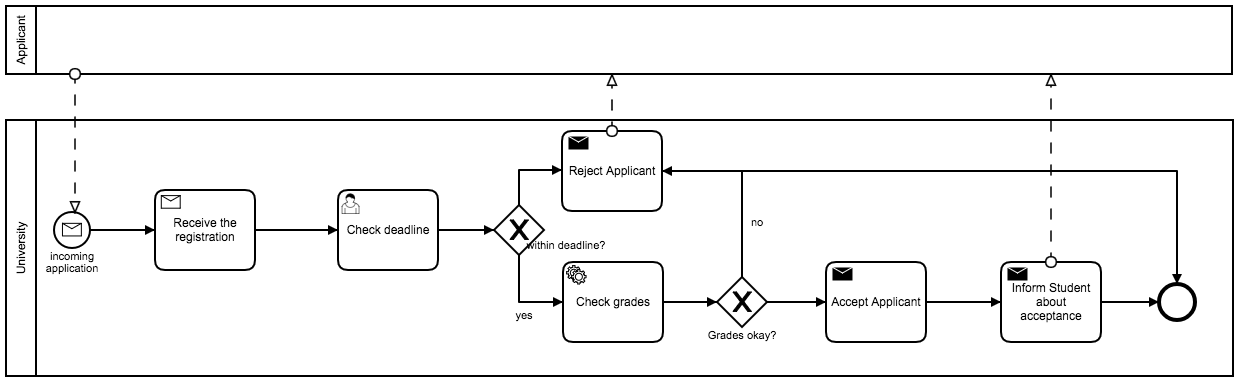
\includegraphics[scale=0.5]{../figures/chapter_indicators/BPMN_Example_Student_Application.png} 
		\caption{A small BPMN example: the application process for study programs.}
	\label{fig:BPMNex}
\end{sidewaysfigure}

Business Process Model and Notation incorporates the term \textit{Business Process}, which has been defined and redefined many times by today. For this thesis, we use the OMG's definition of business processes: 

\begin{quote}
"Business Processes: business plans include Courses of Action - what the enterprise has to do to achieve its Ends - transformed into Business Processes that ecnompass activities, sequencing, dependencies, interactions, triggering by business events, etc." \cite{bmm2015}
\end{quote}

Business processes are ways to achieve goals, to align activities along them and to define interactions, decisions and events. This definition basically incorporates all the core elements of BPMN: activities, paths, swimlanes (for responsibilities), decisions and events. To recap the notation of BPMN, a small example is shown in figure \ref{fig:BPMNex}. \\
In this model, the application process for a student program is shown, which consists of tasks, for instance \textit{Receive the registration} or \textit{Check deadline}. Tasks can be precised as \textit{Manual tasks}, \textit{Send / Receive Tasks} and have assignees, as shown in \textit{Check deadline}. In current workflow management systems, this workflow model can be fully automated and the assignee is presented its tasks when they are instantiated, for example when an application form was received. BPMN models have a start and an end point which can also be events. \newpage
In our example, the starting point is a \textit{Message Event}, that indicates the process has started due to a received message. 
Another major concern in every control flow oriented modeling language are decisions. BPMN models usually consist of several decision points, depicted as diamond-shaped \textit{Gateways}, either empty or with a special symbol inside. Each symbol stands either for \textit{AND}, \textit{OR}, \textit{XOR} or \textit{COMPLEX}. They direct the control flow depending on the decision logic prescribed. In our example, a \textit{XOR} Gateway guides the control flow into either the direction of acceptance or the opposite one, depending on what date the applicant's form was submitted. Additionally, the communication between the workflow's two participants is notated as so called \textit{Pools}, which can be divided into \textit{Swimlanes}. Each pool is a communication partner and a swimlane indicates different responsibilities, such as departments. If a pool is not filled with BPMN elements, the communication partner is out of the modeler's scope and the processes cannot be modeled. These pools are \textit{Black boxes}. \\
As we see in the example, the process is structured and completely predefined, thus has no room for creative decisions or even planning at run-time. The only way the process differs is human intervention or changing the process at design-time. The former is equal to not executing the process in the intended way and the latter is bad for processes in volatile environments. BPMN is suited for a limited variety of processes, foremost business processes and derivatives. The OMG's specification excludes specifically the following \cite{BPMNspec}: 

\begin{quote}

\begin{itemize}
\item "Definition of organizational models and resources,
\item Modeling of functional breakdowns,
\item Data and information models,
\item Modeling of strategy,
\item Business rules models"
\end{itemize}

\end{quote}

%Although excluded, data and information can be modeled by artifacts. It's not like an \textit{Unified Modeling Language} (UML) model where classes and inheritance is mapped, but it is useful to handle forms and different kind of documents which need to be passed along the tasks. 
%For business rules, this is also applicable. BPMN contains a special form of tasks called \textit{Business Rule Task}, which "[...] provides a mechanism for the Process to provide input to a Business Rules Engine and to get the output of calculations that the Business Rules Engine might provide" \cite{BPMNspec}. Business Rule Tasks are predestined for small spreadsheets fed injected into a business rule engine, which is usually a Java class. It is easy to use and implement, since the Business Analyst files a spreadsheet and the developer uses the CSV-file to implement the business rule engine. This procedure, however, works only at design-time and not at run-time, which is a downside being discussed in a subsequent section about DMN. 

% Please add the following required packages to your document preamble:
% \usepackage{booktabs}
\begin{table}[!ht]
\centering
\begin{tabular}{@{}ll@{}}
\toprule
Indicators                   & BPMN                                    \\ \midrule
Documentation style          & Directives                              \\
Preceding process map        & Flowchart                               \\
Characteristics of work      & Routine, predictable, automatable       \\
Characteristics of process   & Rigid, predefined, workflow-centric     \\
Characteristics of decisions & Simple (either / or)                    \\
Control flow                 & Definite control flow, required         \\
Intervention at run-time     & No                                      \\
Objective                    & Automated workflow execution            \\
Type of process              & Business process                        \\
Typical application          & Billing, Accounting, Assembly-line work \\ \bottomrule
\end{tabular}
\caption{BPMN indicators.}
\label{tab:bpmnIndicatorsTable}
\end{table}

Furthermore, the OMG's specification not only provides exclusions such as the ones mentioned above, but it helps to indicate the correct usage of BPMN. Derived from the background chapter \ref{chapter:background} and the example above, the following indicators (table \ref{tab:bpmnIndicatorsTable}) serve as a guidance for modelers to identify when to use BPMN correctly. 

%Information about processes is often stored in documents, deprecated models or held by knowledge carriers according to Dumas et al. \cite{Dumas2013}. This information needs to be extracted by the application of the so called \textit{Process Discovery}, which is in short gathering all the information in a technical or manual way before creating the models. Having this information gathered together, the key question before modeling is \textit{Does the work consist of routine elements which can be optimized or even automated?} (see \ref{tab:bpmnIndicatorsTable}). 
Routine processes occur regularly and their flow is "known a priori" according to \cite{Zeising_2014}. Consequently it is not intended to change the process flow during run-time, as routine ones are well-structured and predefined.\newpage
In our example, the decisions are simple yes or no questions. One of them, \textit{Check grades}, is a business rule task containing a small table of when a grade is acceptable or must be rejected. Overall, the decisions do not require modeling any requirements apart from the assignee involved in the decision making process. Furthermore, the decisions are always stuck with rules or events that happened before. The process itself is control-flow-oriented and the control flow is required and definite since every candidate needs to be processed in a fair and equal manner. In the end, the process could be automated completely with an appropriate workflow management system and would not need any assignee to check the deadline or the grades. In general, BPMN processes are intended to be predictable and to capture routine work. As a matter of fact, a process model's objective is either optimizing or automating a process. In terms of BPMN, the automation of routine work is the main objective although it is not always possible to fully automate business processes. \enlargethispage{1\baselineskip} \\
The given example lacks the documentation and the preceding process map. Both are key artifacts to determine the modeling language, because each contains meta information about the process. Since BPMN processes are often predefined and orchestrated, meaning someone in the company fully designs the process without intended deviation, the documentation resembles directives that are also fully specified and provide a guideline how to correctly execute a task. Directives provide a precise description and strict sequence of tasks along with exception handling and interfaces to different processes. BPMN's core elements are tasks, control flow, events and gateways that are intended to capture the directives and make them executable for machines and human interaction. \enlargethispage{1\baselineskip} \\
A typical application is a billing process or assembly-line work that, in a big picture, results in a certain output creating a value for the company. A billing process can involve several departments and persons of responsibilities. However, every iteration of the process is intended to provide a similar, predictable output and a fully repeatable execution. \\
It is to say that BPMN and DMN resemble a lot when it comes to indicators. The goal of DMN was to create a modeling technique that incorporates both, decision logic and the declarative illustration of dependencies as well as authorities for a decision (see DMN section). The goal was also to create a data handling modeling technique with the ability to process complex rules and data points. Apparently, these decisions are also routine ones and predictable up to a certain point. The main difference between DMN and BPMN is, that DMN is not able to capture workflows and BPMN is not able to capture data processing. As a matter of fact, a combined approach of both modeling techniques might in almost every case be suitable due to the complementary aspect of DMN \cite{DMNspec2016}. 

\section{CMMN and knowledge work}
Routine work occurs in every company, every industry and even in our leisure time. However, not every job is comprised entirely of routine work.
If a person gets sick and needs to see the doctor, often the doctor's job consists of routine and ad hoc parts. Each patient suffers in a different way, has a private or statutory health insurance, is able to understand the doctor's language or not. In each case, the doctor or the medical personnel needs to decide depending on the situation to identify the patient's disease and medicate him accordingly. Overall, this job requires more knowledge and experience than a strict workflow. Applying the BPMN indicators makes the necessity of a different modeling technique obvious, as the indicators do not meet the requirements of this example (adaptable instead of a definite workflow, knowledge-centric process instead of workflow-centric).\\
Standardized by the OMG in 2014 \cite{CMMNspec2014}, the modeling language is intended to meet the requirements of knowledge intensive professions and support workers with models and their execution in workflow management systems. 
The previously described example differs from the business processes explained in the BPMN section earlier. Instead of focusing on what \textit{has} to be done in which order, the medical personnel should adhere to what \textit{can} be done, as Van der Aalst et al. described in \cite{aalst2005}. This is an essential part of the \textit{Case Management} (CM) and \textit{Adaptive Case Management} (ACM) approach.\\
 Case management starts with a case such as a legal case, a patient's disease or "some other focal point around which actions are taken to achieve an objective" \cite{CMMNspec2014}. As a matter of fact, a case can also be a project that has to be managed or an event that needs to be organized. \\
Each case contains a set of tasks and files necessary to achieve the goal. These sets are "minimally predefined" \cite{CMMNspec2014} resulting in two phases of working with cases: the design phase and the running phase \cite{CMMNspec2014}. During the design phase, tasks and information are aggregated in a manner that is very similar to business process designs. As a result, the work is available in a more structured way than it has been before, yet with the possibility to perform the work completely situation-dependent, if necessary. Case management requires the run-time flexibility such as performing tasks depending on the situation, changing the order of tasks or even collaborate with different people involved as intended. \\
At a first glance, this seems counter-intuitive to the common understanding of modeling processes, which is often modeling business processes or similar strictly structured ones. To illustrate the paradigm of case management and introduce the CMMN notation, figure \ref{fig:CMMNex} provides an example. The subsequent explanation is derived from \cite{CMMNspec2014} and \cite{hinkelmann2015}.

\begin{sidewaysfigure}

	\label{fig:CMMNex}
	\centering
	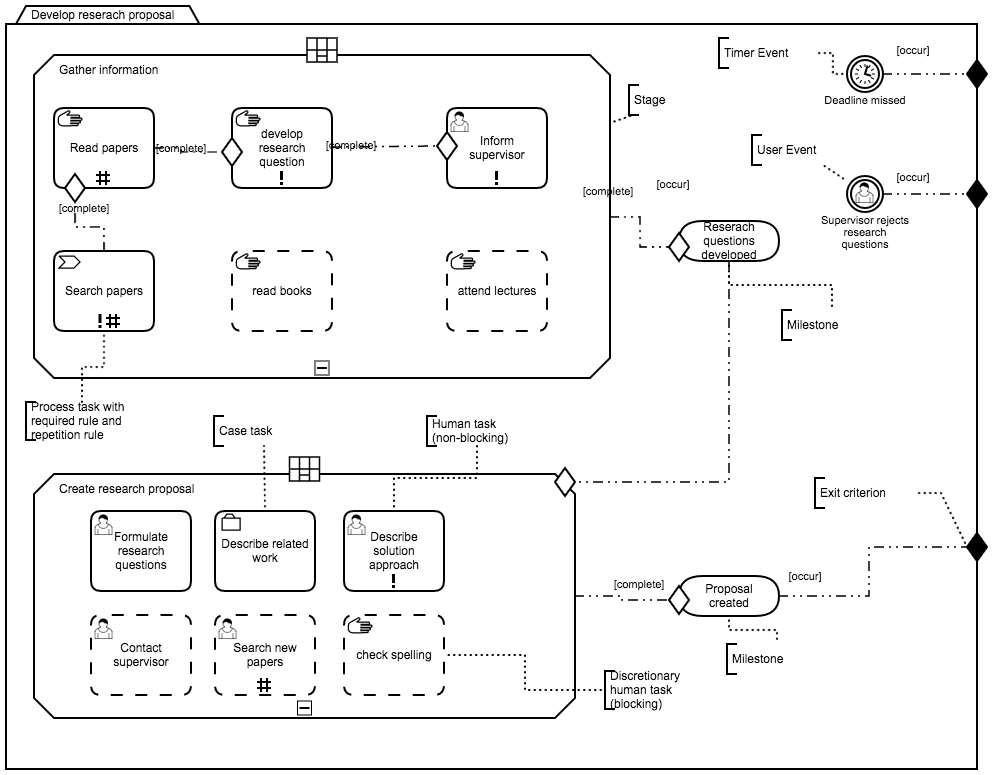
\includegraphics[scale=0.5]{../figures/chapter_indicators/CMMN_Example_Proposal_Creation.png} 
		\caption{CMMN example: Creating a research proposal.}
\end{sidewaysfigure}

The first element that immediately catches the eye in this example is a large folder depicting the \texttt{Case Plan Model}, a root element containing all further elements involved with a name tag in the upper left corner. Next, there is a big structure called \textit{Stage}, illustrated as a rectangle. Similar to BPMN, stages form a group of elements into a sub process or - to put it in the CMMN context - in a sub case. Stages can be connected via \textit{Sentries} and \textit{Connectors} that are the lines between \textit{tasks} and the diamond shaped \textit{exit or entry criteria}. Both, exit and entry criteria trigger when \textit{events} occur. There are three rules to make sentries trigger:

\begin{itemize}
\item \texttt{on [event] if [condition]} 
\item \texttt{on [ event]}
\item\texttt{if  [condition]}
\end{itemize}

According to the CMMN specification, this provides the opportunity to receive events and check whether they have effect on the following process steps \cite{CMMNspec2014}. \\
In figure \ref{fig:CMMNex}, a timing event is called \textit{Deadline missed}. This event is connected to an exit criterion, denoted as a black diamond on the border of the Case Plan Model. \newpage When the event is triggered, the sentry checks \texttt{on [deadline missed] if [date today > deadline date]} and triggers the exit criterion terminating the case due to the missed deadline. A different event type is the \textit{User Event}, listening to user interactions that trigger the exit criterion. Besides these two event types, each task, stage and \textit{Case File Item} can trigger events on their own, which are received by sentries. \textit{Case File Items} are containers for pieces of information, for instance the patient's record or in this example the papers, which need to be read (not contained in the diagram). They are denoted as documents, similar to the shape of a document icon on a personal computer.\\
Another structural element is the \textit{Milestone}, an oval shaped form representing an "achievable target" \cite{CMMNspec2014} and providing the ability to measure the progress of a case. Each milestone can have multiple entry criteria or none to show that a milestone is reached or not. In general, "no work is directly associated with a milestone" \cite{CMMNspec2014} but rather a "completion of a set of tasks" or "the availability of key deliverables" \cite{CMMNspec2014}. \\
Figure \ref{fig:CMMNex} contains two example milestones: \textit{Research questions developed} and \textit{Proposal created}. Both milestones are connected to either a stage or an exit criterion indicating a dependency. The first milestone needs to be achieved to create the research proposal, the latter one determines the successful termination of the case. \\
As mentioned earlier, CM requires run-time flexibility and by now, there has nothing been explained but tasks, events and milestones which are per se inflexible. To guarantee run-time planning, tasks and stages have a discretionary version. Discretionary means, a user may decide during run-time if this task or stage will be executed in a following iteration. This mechanism makes it possible to model knowledge and experience combined with routine steps. In our example, the gathered papers might not be enough to provide good citations and emphasize the solution approach. Here, only the case worker can identify if he needs to do more research to find correct citations, as this is a decision requiring knowledge and experience in writing research papers. It is up to his or her discretion if the task will be executed or not. \\
Supplementary to \textit{Discretionary Items}, \textit{Planning Tables} indicate the ability to plan Discretionary Items and apply control mechanisms called \textit{Applicability Rules}. Case workers are presented \textit{Planning Items} if the corresponding Applicability Rule evaluates to true. Overall, this allows the modeler and the case workers to plan at design-time (creating the case model) and at run-time (planning the time discretionary items). \newpage
The last visible part of the CMMN notation that has not been explained, is the type of tasks available. In the example case, there are four types of tasks (each type can be indicated in the upper right corner of the task):

\begin{itemize}
\item \textit{Human Tasks} either blocking (indicated with a "User" in the upper right corner) or non-blocking with a hand in the right corner
\item \textit{Process Task} with a "Chevron" symbol 
\item \textit{Case Task} with a folder symbol 
\end{itemize}

Both Human Tasks indicate that an assignee with the appropriate role needs to fulfill the modeled work here. \textit{Non-blocking} signifies this step can be done while other tasks of the model run simultaneously. \\
In contrast, the blocking one does not allow other tasks to be performed at the same time. A \textit{Process Task} calls a business process, modeled, for example, in BPMN and a \textit{Case Task} calls a different case, handing over input parameters and demanding an output. \\
In figure \ref{fig:CMMNex}, \textit{Read papers} is a non-blocking human task, \textit{Read books} a non-blocking discretionary human task, \textit{Frame research questions} a blocking human task, \textit{Describe related work} a case task and \textit{Search papers} a business process task.\\
Apart from the mentioned types of tasks, there a additional execution semantics as seen in the \textit{Search for papers} task. An exclamation mark signifies this task has to be performed, a sharp mean this task has several iterations and a play symbol indicates the \textit{Manual Activation Rule} (not in the example). This rule is connected to entry criteria and transitions from the status \texttt{enabled} to \textit{active} if the criterion's condition is fulfilled. \\
CMMN, in contrast to BPMN, offers a complete lifecycle with corresponding states.

\begin{figure}
  \centering
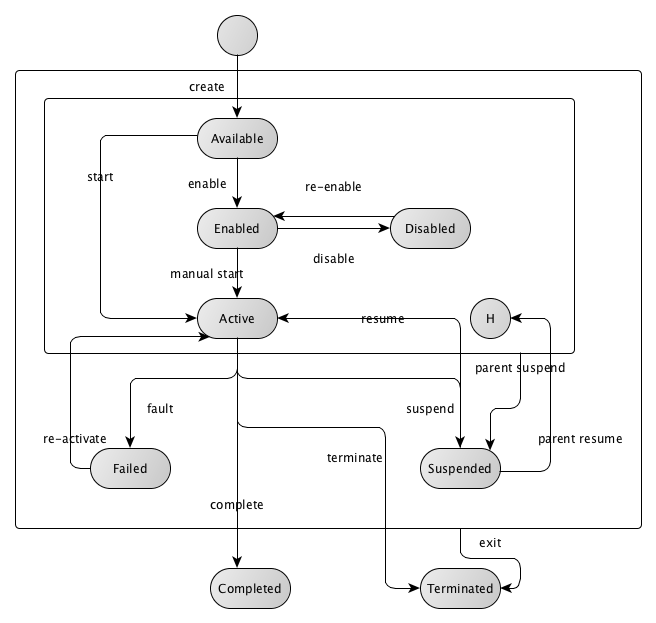
\includegraphics[width=0.7\textwidth]{../figures/chapter_indicators/CMMN_Stage_and_Task_Lifecycle_CMMN.png} 
\caption{Stage and Task Lifecycle adopted from Figure 7.3 in the CMMN specification \cite{CMMNspec2014}.}
  \label{fig:CMMNstates}
\end{figure}

Figure \ref{fig:CMMNstates} is a replica of Figure 7.3 in \cite{CMMNspec2014} and shows the different states and transitions for stages and tasks. These stages allow modelers and workers to measure and plan work in a different way as with BPMN. \\
One of BPMN's commonly mentioned downsides is the lack of states and transitions according to \cite{Recker2010}. In the example (Fig. \ref{fig:CMMNex}), states are not included since they are not visible in the notation and only occur during run-time. In addition to Fig. \ref{fig:CMMNstates}, CMMN offers similar states for sentries and the whole case plan model and can be found in the execution semantics chapter in \cite{CMMNspec2014}. \newpage

% Please add the following required packages to your document preamble:
% \usepackage{booktabs}
% \usepackage{graphicx}
% \usepackage[normalem]{ulem}
% \useunder{\uline}{\ul}{}
\begin{table}[]
\centering
\resizebox{\textwidth}{!}{%
\begin{tabular}{@{}ll@{}}
\toprule
Indicators                   & CMMN                                                 \\ \midrule
Documentation style          & Descriptions of best practices and recommendations   \\
Preceding process map        & Cluster                                              \\
Characteristics of work      & Agile, emerging, not automatable                     \\
Characteristics of process   & Adaptive, partly predefined, knowledge-centric       \\
Characteristics of decisions & Stateful (transition form one to another state)      \\
Control flow                 & Indefinite control flow, optional                    \\
Intervention at run-time     & Yes                                                  \\
Objective                    & Support manual work                                  \\
Type of process              & Case                                                 \\
Typical application          & Reviews, Medical attendance, Managing and organising \\ \bottomrule
\end{tabular}%
}
\caption{CMMN indicators.}
\label{tab:CMMN_indicators}
\end{table}

Table \ref{tab:CMMN_indicators} summarizes the notation's characteristics and classifies them as indicators. In the earlier examples, we saw that CMMN is suitable for agile and partly predefined work. The worker's knowledge is crucial during the execution phase, whereas workflows and sequences are less important. Compared to BPMN, CMMN captures the flexibility of processes that require situation-dependent decisions, agile work whose tasks emerge during run-time and cannot, or at least to a small extent, be predicted and thus predefined during design-time. Furthermore, decisions are stateful due to rules and sentries, and serve as monitoring tools instead of sequencing work. This leads to a flexible control flow, only describing the dependencies of task or milestones that need to be achieved in order to fulfill the whole case. \\
CMMN documentation and process maps might resemble best practices or descriptions of work, as the content of cases often diverges. However, process discovery should lead to some extent of a description, what can be done to achieve the case and what are the key elements that need to be modeled. Following this, process mapping would rather result in an aggregation of tasks that belong together instead of a flowchart indicating steps and sequences. \\
Overall, BPMN and CMMN differentiate in many points and capture completely different settings. BPMN has the objective to automate processes, whereas CMMN is intended to support workers by automating certain steps or simplifying the monitoring of a case. This makes it a declarative modeling technique according to \cite{FahlandLuebkeMendlingEtAl2009}. 

%Table \ref{tab:cmmnIndicatorsTable} shows a summary derived from the explanation and the example, both planting on the basis of the CMMN specification \cite{CMMNspec2014}. The example emphasized that CMMN is in general applicable for not predefined, to a high degree knowledge dependent work. Decisions are modeled in conditions on when to enter or exit stages, task or milestones. Rules such as \textit{Application Rule} or \textit{Repetition Rule} allow the modeler to guide the case worker through tasks and show him or her what tasks have to be done and which have to be done for a specific amount of iterations. However, decisions similar to gateways in BPMN are not in scope of this notation and dedicated to the case worker. In addition, the required flexibility is fulfilled by \textit{Discretionary Items} allowing the workers with the appropriate role to adapt the workflow in during run-time. States as shown in figure \ref{fig:CMMNstates} contribute to this flexibility but also let the involved personnel measure the progress of each case. This results in a more manageable and verifiable way of Case Management. 

\section{DMN and decision making}
In section \ref{section:BPMNindicators}, decision-making in BPMN was shown with the aid of a small example, whose excerpt is shown in figure \ref{fig:BPMNshortenedApplicationEx}. Two gateways guide the control flow according to the decisions made. Each gateway compares a value with a given limit and verifies it. If the value is withing the limitation, the control flow passes on to the next gateway or, in case the value is out of bounds, rejects the student's application. These are simple \textit{either or} questions. \\
Figure \ref{fig:BPMNexpandedApplicationEx} demonstrates a more sophisticated version of the same process. To pass the application process,  one of the four requirements needs to be fulfilled. Each requirement is implemented as a gateway that checks if the applicant either fulfills it or not. All of the gateways are \texttt{OR} gateways, signalizing a lose decision making compared to \texttt{XOR} gateways. At a first glance, figure \ref{fig:BPMNexpandedApplicationEx} looks more complicated than figure \ref{fig:BPMNshortenedApplicationEx}. Although the actual decision-making process is kept simple, the BPMN notation with its gateways makes it look confusing and, at a much larger scale, for the reader impossible to comprehend the process as a whole. At this point, DMN becomes relevant. \\

The DMN notation comprises two parts: the \acl{DRG} with one or more \aclp{DRD} and the decision tables. Figure \ref{fig:DMN_DRD_Application} illustrates the corresponding \ac{DRG} for the decision-making seen in Fig. \ref{fig:BPMNexpandedApplicationEx}. Moreover, DMN's notation for DRDs contains only four distinct shapes and three different types of connectors, which can be seen in Fig. \ref{fig:DMN_DRD_Application}: 

\begin{itemize}
\item \textit{Decision}: Decisions are depicted as rectangles and incorporate the decision logic which is mapped in decision tables. In the example, there are two decisions: \textit{Deadline check} and \textit{Acceptance rate according to Transcript of Record}. Both have a table symbol in the upper right corner indicating the decision logic. 
\item \textit{Input Data}: Each decision needs inputs. \textit{Input data} is the fundamental and least complex form possible. This element stores information of any type, from simple types like dates and integers to lists and functions expressed via \acf{FEEL}. An \textit{Input Data} element may only be connected directly to decisions and knowledge sources. 
\item \textit{Knowledge Source}: DMN makes it explicit where knowledge sources are involved in the decision-making. Typically knowledge sources are documents, best practices, but also people or bodies of legislation \cite{DMNspec2016}. "Knowledge sources are the authorities for a decision [...]" \cite{DMNmicroguide}, which may be connected with input data, since managers, for instance, might need background information not directly involved in the decision logic. In the example, the application policy and annual plan of the university is used as \textit{knowledge source}.
\item \textit{Business Knowledge Model}: In contrast to Knowledge Sources, Business Knowledge Models are non-authoritative and serve as container for analytic models, decision logic or business rules \cite{DMNspec2016}. It is depicted as a rectangle with cut-off corners in the upper left and lower right. As they only influence decisions directly, the specification allows consequently no connection but with decisions or different business knowledge models. Due to the shortness of the example, Business Knowledge models are not contained in Figure  \ref{fig:DMN_DRD_Application}. 
\end{itemize}

\begin{sidewaysfigure}[]
  \centering
    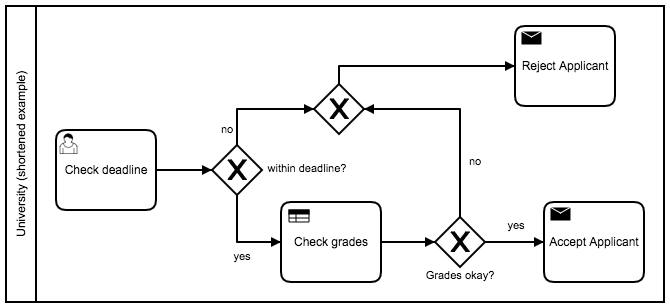
\includegraphics[scale=0.5]{../figures/chapter_indicators/BPMN_Example_Student_Application_Short.png}
    \caption{Shortened example from section \ref{section:BPMNindicators} with only two decisions.}
  \label{fig:BPMNshortenedApplicationEx}
    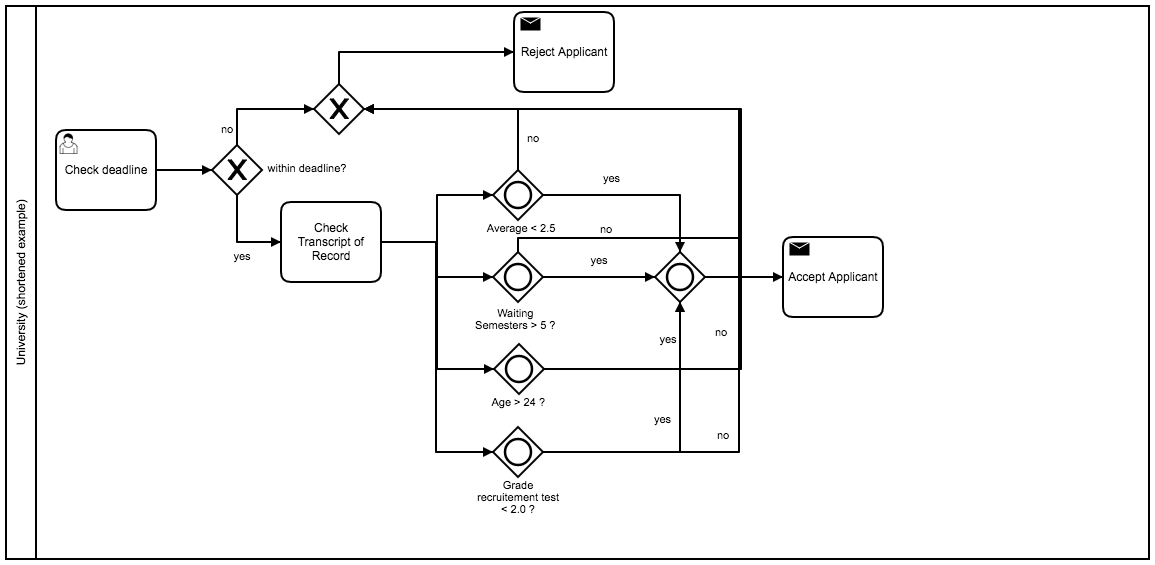
\includegraphics[scale=0.4]{../figures/chapter_indicators/BPMN_Example_Student_Application_DMN_Short.png}
    \caption{Shortened example from section \ref{section:BPMNindicators} with additional decisions.}
  \label{fig:BPMNexpandedApplicationEx}
\end{sidewaysfigure}

\begin{figure}[!h]
\begin{center}
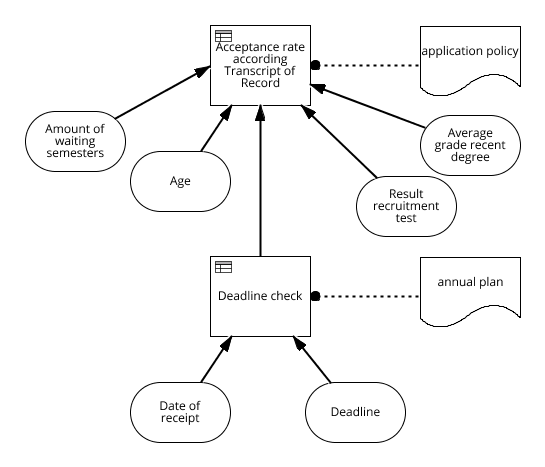
\includegraphics[width=0.5\textwidth]{../figures/chapter_indicators/DMN_Application_Example_Deadline_ToR.png} 
\end{center}
\caption{A DMN Decision Requirement Graph incorporating the decision-making of the BPMN process in \ref{fig:BPMNexpandedApplicationEx}.}
\label{fig:DMN_DRD_Application}
\end{figure}

\begin{sidewaysfigure}
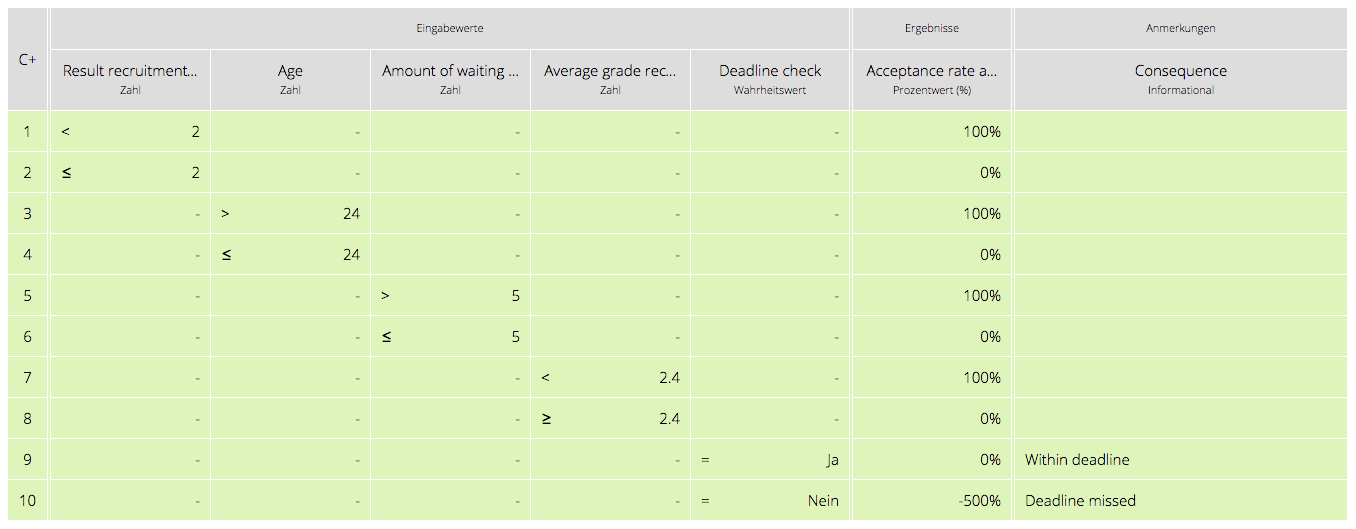
\includegraphics[width=\textwidth]{../figures/chapter_indicators/DMN_Application_Example_Decision_Table_ToR.png} 
\caption{An example DMN decision table with the decision logic accord to the BPMN example in Fig. \ref{fig:BPMNexpandedApplicationEx}.}
\label{fig:DMN_decision_table_application}
\end{sidewaysfigure}
As stated above, the notation comprises only four elements making it a very compact modeling language in terms of the \ac{DRG}. In addition, there are three different connectors indicating either an \textit{information requirement} (connections from decisions to decisions or input data to decisions), an \textit{authority requirement} (connections from knowledge models to decisions, business knowledge models or different knowledge sources) or \textit{knowledge requirement} (connections from business knowledge models to decisions or different business knowledge models). \\
The second part of the DMN specification allows the modeler to create decision tables containing the decision logic. An example table \footnote{Each modeling tool implementing the DMN specification is allowed to vary the orientation of decision tables and the concrete look, for instance colors or shades.} is provided in Figure \ref{fig:DMN_DRD_Application}, implementing the decision logic according to the BPMN example in Figure \ref{fig:BPMNexpandedApplicationEx}. Each table is comprised of several input columns and at least one output column. An input can be a string, integers, floats or basically any type of numbers or enumerations. In this example table, there are five input columns and one output column with annotations such as \texttt{Deadline missed}. Each row signifies a rule in the following syntax: \texttt{If [INPUT A] AND [INPUT B] then [OUTPUT C]} \cite{DMNspec2016}. \\
The inputs are logically connected by the boolean \texttt{AND}-operator, resulting in as many outputs as desired, if a rule matches. For every input in the decision table, there is an \texttt{input data} element modeled in the related \ac{DRG}. This also applies for decisions and sub-decisions. \\
Comparing the table with the BPMN example demonstrates a downside of the decision table: the "\texttt{AND} only" syntax. However, modeling \texttt{OR} connections is possible with a workaround. \newpage Besides the table's data and rules, business analysts can also define \textit{hit policies}. These policies are necessary if some of the rules overlap. In the example table (Fig. \ref{fig:DMN_DRD_Application}), all of the rules are intended to overlap making a hit policy necessary. There are two major categories of policies: \texttt{single hit} and \texttt{multiple hit}. The former one allows only to trigger one rule, the latter one allows several rules to trigger. A brief overview with an explanation can be found in table \ref{tab:DMN_hit_policies}. 

% Please add the following required packages to your document preamble:
% \usepackage{booktabs}
% \usepackage{graphicx}
\begin{table}[]
\centering
\resizebox{\textwidth}{!}{%
\begin{tabular}{@{}ll@{}}
\toprule
Policy       & Variations                                                                                                             \\ \midrule
Single hit   & Unique (no overlap allowed)                                                                                            \\
             & Any (overlap allowed, outputs must be equal)                                                                           \\
             & Priority (returns matching rule with highest output priority)                                                          \\
             & First (first hit by rule order)                                                                                        \\
Multiple hit & Output order (returns all hits in decreasing output priority order)                                                    \\
             & Rule order (returns all hits in rule order)                                                                            \\
             & \begin{tabular}[c]{@{}l@{}}Collect (aggregates all hits with specified operators:\\ sum, min, max, count)\end{tabular} \\ \bottomrule
\end{tabular}%
}
\caption{DMN hit policies cited from the DMN specification \cite{DMNspec2016}.}
\label{tab:DMN_hit_policies}
\end{table}
 
To achieve an \texttt{OR} connection of the rules, the hit policy is set to \texttt{Multiple Hit: collect (sum)} and the measuring unit of the output is set to percentage. Consequently, the acceptance rate is measured in percentage. The applicant is able to achieve zero or more than 100 percent according to the \texttt{collect: sum} rule. Another problem of this method is the inflexibility of the outputs. In this example, an output value of \texttt{true} or \texttt{false} would have been the best way to model the decision, but neither the decision table, nor \acl{FEEL} allow the aggregation of boolean values. \\
To individualize the decision logic or create more advanced rules, the DMN specification aggregates functions and types into an expression language called \ac{FEEL}. \newpage
FEEL is similar to \ac{SQL} and \ac{PMML} \cite{DMNspec2016}, making it easier to understand for non-developers. The expression used in the \texttt{deadline check} table is also a predefined function with two input parameters (deadline date and date of receipt) and a range of numbers implemented implemented as two rules: \texttt{DayDiff(Date of receipt, Deadline)}. \\
The last one to mention here is the sub-decision \texttt{Deadline check}. The decision logic is not implemented in this table, but is referenced by a another decision table (see Fig. \ref{fig:DMN_DRD_Application} for illustration). A simple check written in \ac{FEEL} counts the difference between the application's date of receipt and the given deadline. If the result is less than zero, the deadline is missed and the output of \texttt{Deadline check} is \texttt{false}. Otherwise, if the result equals zero or more, it evaluates to \texttt{true}. \\

To recap, the examples illustrated the multiple uses of the DMN language. Decision tables are useful for automating data intensive decisions and replacing vast BPMN gateway trees. In the same way, it is possible to model decisions that require rather knowledge, best practices or analyses than a large amount of data by skipping the decision logic part and only define the dependency graph. \\
On the contrary, it is not possible to model any sequence with the DMN notation apart from the dependency of decisions or the amount of iterations. Although the specification emphasizes the independence of the notation \cite{DMNspec2016}, the \ac{DRG} on its own might have few useful cases of application where a standalone \ac{DRG} is the most convenient solution. \\

% Please add the following required packages to your document preamble:
% \usepackage{booktabs}
% \usepackage{graphicx}
\begin{table}[]
\centering
\resizebox{\textwidth}{!}{%
\begin{tabular}{@{}ll@{}}
\toprule
Indicators                   & DMN                                                       \\ \midrule
Documentation style          & Spreadsheets                                              \\
Preceding process map        & Decision trees                                            \\
Characteristics of work      & Decision-intensive, data handling, decision-making              \\
Characteristics of process   & Complementary, data processing, data-centric                        \\
Characteristics of decisions & Complex (data processing)                                 \\
Control flow                 & Dependencies, required                                    \\
Intervention at run-time     & Yes                                                       \\
Objective                    & Automated data processing                                 \\
Type of process              & Decisions                                                 \\
Typical application          & Calculation of discount rates, salary, choosing assignees \\ \bottomrule
\end{tabular}%
}
\caption{Indicators for the identification of DMN use cases.}
\label{tab:DMN_indicators}
\end{table}

Table \ref{tab:DMN_indicators} summarizes the knowledge acquired by analyzing the DMN specification \cite{DMNspec2016}, Debevoise and Taylor \cite{DMNmicroguide} and \cite{BiardMauffBigandEtAl2015a}, as well as creating the provided examples in this section. It was shown that DMN is an applicable solution for processes that focus on decisions, thus are complex to illustrate in BPMN. The most common applications are calculations of salaries, provided in \cite{DMNspec2016}, or making a choice by several influencing factors, for instance choosing the right vehicle for hazardous material \cite{DMNmicroguide}. Particularly the breakdown into two parts, the \acl{DRG} and the decision tables, makes it simple for the modeler to decide between decisions that only need data (therefore use the decision table), model the dependencies of decisions and the decision-makers (ergo utilize the \ac{DRG}), or combine both. \\
Table \ref{tab:DMN_indicators} also shows a similarity to BPMN: Both modeling approaches aim at the automation of their domains. BPMN's objective is to automate workflows, whereas DMN provides the ability to automate decisions. Both notations capture routine work that is mostly predefined. In addition to that, DMN provides the ability to adapt values of the decision logic during run-time. How this is exactly achieved depends on the implementation by the corresponding software tool. Camunda, for example, provides a \ac{REST} API that allows the users to create or delete decisions during run-time. \\
The main difference between DMN and BPMN, however, is what they are able to capture. DMN is a notation that is only able to to process data and to output a decision that can be handled by other modeling languages, if desired. BPMN is also able to handle decisions, but not to process data in the way DMN does. \newpage This is emphasized by the control flow of the DMN language: Decisions can be enhanced with dependencies and knowledge sources. Overall, DMN is a notation that only serves for decisions and does not work for any different use case. \\
Data that needs to be processed to find a decision is often stored in spreadsheets instead of free text documents. This is a strong indicator for DMN, since the spreadsheets can be transferred into DMN's decision logic. Furthermore, decisions that have sub-decisions or dependencies might be clustered in a decision tree during process discovery. The \ac{DRD} is able to incorporate these decision trees and make them executable. \\
In Chapter \ref{chapter:combination}, the combination of DMN and BPMN is described along with use cases where DMN is suitable as a replacement for gateways and functions as a data processor or event-handler. This chapter describes the complementary character of the DMN notation as well.


\section{Summary}
In this chapter, each specification was presented with examples and their characteristics. By analyzing the OMG's standards and further research publications, these characteristics could be transformed into indicators helping modelers to identify when to use the corresponding technique. The examples explained the fundamental principles of the notations and how to use them correctly. The main focus, however, was developing the indicators. For further information about the notations and more sophisticated examples or instructions, please refer to the corresponding OMG specification or the provided sources in the references chapter. \\
A recommendation of how to combine manual process discovery techniques was presented along with an explanation of each approach. Besides the manual discovery, the automated one was illustrated and a recommendation for a corresponding tool was outlined. \\
Concluding the indicator sections, BPMN is useful for predefined processes, mainly mapping routine work without the possibility for run-time intervention. CMMN is suitable for people working in volatile environments with routine parts, but mainly work depending on their personal experience and knowledge. DMN is a valuable way to encapsulate complex, data-intensive decision-making in a separate, compact notation that allows run-time adjustments. For all of the mentioned notations, there are overlaps that make it possible to combine them and creating a whole model with separate notations for each domains. This will be discussed more detailed in the following chapter.

\part{Combination}
\label{part:combination}
\chapter{Combining the different standards}
\label{chapter:combination}
\lstset{
  language=XML, escapechar=|,
  morekeywords={encoding,
    xs:schema,xs:element,xs:complexType,xs:sequence,xs:attribute}
}

In the previous chapter, indicators were presented to distinguish between the standards and to identify when to use the corresponding one for a given use case. Some cases, however, require a combined use of the presented models to achieve run time flexibility in BPMN models, or to represent routine parts in a flexible CMMN model. An explanation, when to combine models and how to combine them is presented in this chapter. 
\section{When to combine}
The indicators in Chapter \ref{chapter:indicators} provide a set of characteristics to differentiate between the three named specifications: DMN, CMMN and BPMN. This is useful for rather small processes with exactly defined purposes and without any exception handling or interfaces to external processes. However, processes might become larger and thus harder to understand. In addition, process models can become biased by human error and cause performance issues, apart from the inability to model certain scenarios with only a single notation. Besides the performance, small processes are often part of a larger process landscape which need to be integrated somehow. Consequently, there have to be  interfaces for inter-procedural communication and modeling tools that support inter-procedural modeling. \\

When to combine different modeling approaches is a question, that needs to be answered for every use case. The indicators in Chapter \ref{chapter:indicators} provide a set characteristics supporting the decision, when to use the corresponding modeling approach correctly. At this point, the so called \textit{Separation of concerns} \cite{BiardMauffBigandEtAl2015a} comes into play, meaning each modeling language has a domain, where it suits best. DMN is best for decisions, BPMN for routine and CMMN for unpredictable work. Separating the concerns means, in a transferred sense, to divide the discovered information into parts and domains that can be modeled with the correct modeling language. \\
Process discovery aims, as explained in a preceding chapter, to identify individual processes and their tasks.\newpage These processes form small, definite units, similar to decoupling in software engineering. Each process should represent a logical unit that can be inter- and exchanged in a larger process landscape. Forming such a landscape consequently leads to a high degree of decoupling and functional cohesion. As a matter of fact, this is the  realization of \textit{separating the concerns}. \\
To achieve a high degree of decoupling and a functional cohesion, the process discovery first needs to define small processes encapsulating one logical unit. Second, the indicators should be applied to identify the correct modeling language. Finally, the composition of a larger process model can be done by integration of the small units with interface tasks. This last step is discussed in the subsequent sections. 
%To achieve a separation of concerns, the analyst need to focus on dividing tasks and steps in separate models. With the provided indicators from Chapter \ref{chapter:indicators} it is possible aggregate process tasks or steps into a  
\section{Combining CMMN with BPMN}
To illustrate the benefits of a BPMN and CMMN combination, we construct a practical scenario of a bank and a customer who wants to open a new bank account. One of the very first steps is to verify the customer's identity. Of course, this process can be done in a branch office where an employee checks the customer's identity card. However, some banks rely on online procedures with photos and codes to fasten up this procedure.\\
Apparently, the largest part of this procedure should be repeatable and follow a strict routine to validate the identity. Consequently, the main process should be modeled in BPMN. However, each process is error-prone, leading to exceptions. In our example, call center agents are supposed to handle these exceptions. At a first glance, call center agents work partly routine and partly depending on the circumstances. A look at the indicators identifies CMMN as the right modeling language for this purpose. Finally, these exceptions can be modeled in CMMN and linked to the BPMN model. 
 \\
This short example shows a possible combination of two models. The online process is designed and modeled in BPMN due to the vast amount of routine steps. The agent's call is more of a knowledge task he has to do. It comprises routine parts and discretionary items such as answering questions or fixing problems posed by the customer. Consequently, a combination of CMMN and BPMN suits best for this use case. 

\begin{figure}
  \centering
    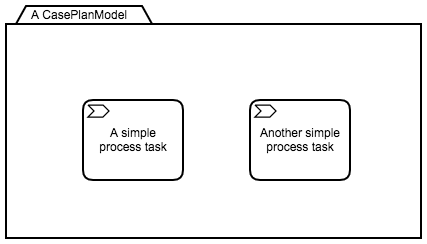
\includegraphics[width=0.7\textwidth]{../figures/chapter_combinations/CMMN_Process_Tasks.png}
      \caption{A CMMN process task to call a BPMN process.}
      \label{fig:CMMN_process_task}
\end{figure}

There are two ways of combination: integrating CMMN in a BPMN model and the opposite way. 
Figure \ref{fig:CMMN_process_task} illustrates a simple Case Plan Model containing two tasks: \textit{A simple process task} and \textit{Another simple process task}. Both "[...] can be used in the Case to call a Business Process" \cite{CMMNspec2014}.\\\\
As the CMMN specification stated, this is a \textit{call activity} with the intention to direct the process into another (sub-) process. A brief look at the meta model proves this hypothesis by the following attributes of the CMMN process task: \texttt{implementationType : URI}\footnote{Read \textit{<attribute> : <type>}}, \textit{inputs : ProcessParameter} and \textit{outputs : ProcessParameter} \cite{CMMNspec2014}. The \textit{implementationType} attribute indicates the link to other processes, namely \ac{BPMN}, \ac{XPDL} version 2.x, \ac{WSBPEL} 2.0 and  \ac{WSBPEL} 1.0. The called processes are handed over zero or more input parameters and return the results as output parameters, subsequently processed by the main process. \\
How this link between both models is visually presented depends on the tool the analyst uses. Camunda, for example, uses attributes to link the processes. Signavio links the models directly, so the user only has to click the process symbol in the upper right corner of a process task to switch the models. Though, it is not possible to explicit model BPMN in the CMMN notation, which holds for all notations: BPMN, CMMN and DMN. It is possible to link them, but not to create BPMN models with e.g. the notation set of CMMN. As CMMN is a fairly new specification, the way how combined models can be presented to the user might vary until the tools support the standard completely. \newpage

\begin{figure}
  \centering
    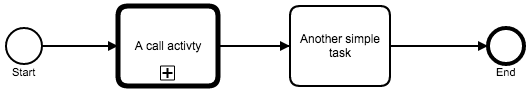
\includegraphics[width=0.7\textwidth]{../figures/chapter_combinations/BPMN_Call_Task.png}
      \caption{A BPMN model with a call activity and an unspecified task.}
      \label{fig:BPMN_call_activity}
\end{figure}

In Fig. \ref{fig:BPMN_call_activity} a very small business BPMN process is shown. It comprises a \textit{call activity} and a very simple \textit{task}. Here, the call activity is able to integrate a CMMN model. According to the BPMN specification, "a call activity identifies a point in the process, where a global process or a global task is used" \cite{BPMNspec}. \\
Again, the meta model proves the ability to link different processes. A Call activity has an attribute \textit{calledElement: CallableElement} that instantiates an object of the super class \textit{CallableElement}. This super class provides an \textit{ioSpecification} and an \textit{ioBinding} attribute, as well as a specification of the used interface. Eventually, the \textit{ioBinding} allows to define the inputs and outputs as well as one or more operations on the data sets. The \textit{ioSpecification} is used to specify the inputs and outputs of the activity, whereas the \textit{ioBinding} becomes necessary when the Call Activity is linked to a service instead of a process \cite{BPMNspec}.
Consequently, a globally defined\footnote{Globally defined means the called object is not a sub-object that can only be instantiated with the main object. Globally defined objects can be called and instatiated.} CMMN case (which can also referred to as a process) can be called here. As the call activity is not a native CMMN-link, the \textit{CallActivityType} needs to be set to CMMN. Each call activity has to deliver an output value that is generated during the execution \cite{BPMNspec}. When invoking a process it is necessary to keep in mind that a call activity is able to override the attributes of a called process. Consequently, the behavior of the called process might change \cite{BPMNspec}.\\

In BPMN, a token traverses the model. Each gateway either directs the token to another direction or even multiplies it (\textit{AND} gateway). At each endpoint of the process model, only one token arrives and ends the instance of the process. By inserting a call activity in BPMN, the token is blocked until the called process ends and escalates the result to the calling process. Consequently, the called process could call another one and this one could also call a process, leading to a huge capacity usage and consequently to an abortion of the instance. To avoid this situation, BPMN provides the \textit{Termination Event} that, when reached by a token, terminates the process immediately and discards the other tokens.

\section{Combining DMN with BPMN}
The "DMN notation is designed to be usable alongside the standard BPMN business process notation", states the first paragraph in the DMN specification \cite{DMNspec2016}. Consequently, DMN serves as a complementary language to BPMN and helps to "[...] create lighter, more focused processes by moving decision details into DMN" \cite{DMNmicroguide}. This leads to a clear structure without a vast amount of gateways and faster processing. Generally speaking, the standalone version of DMN is useful for modeling decisions and their requirements with the \ac{DRG}. The benefits of DMN can be used to a full extent, however, by combining it with another modeling language, for instance BPMN. \\
BPMN has one designated interface for DMN decision logic and several more or less suited ones. Table \ref{tab:BPMN_elements_DMN_compatibility} shows BPMN's interface tasks explained by the DMN specification. It stands out that the Business Rule Task is the designated interface, since the BPMN specification defines it as a "[...] mechanism for the Process to provide input to a Business Rules Engine and to get the output of calculations that the Business Rules Engine might provide" \cite{BPMNspec}. As a matter of fact, this is the main purpose of the DMN notation. \\
Figure \ref{fig:DMN_table_in_BusinessRuleTask} illustrates the combination of a BPMN model and the DMN decision logic and how it is implemented by the signavio modeler. The Business Rule Task has an attribute that links to the DMN model and calls the decision with the input parameters. According to the decision logic, the parameter is matched with the correct rule leading to the desired output. In this example, the salary of an employee along with additional privileges needs to be calculated. Obviously, this seems to be a predefined and fully repeatable task combined with a data-centric decision. Although it is possible to model both characteristics in BPMN, it is better to separate them according to their concerns. This leads to simpler models and better performance. \\
The example company has three different roles: executives, knowledge workers and routine workers. Each position is paid accordingly and gets an additional privilege. The executive, for instance, gets a salary of 3000 EUR. coupled with a company vehicle. In BPMN, the process sends the parameter to the decision engine and returns the right salary, which is paid after the calculation. The payment procedure is denoted as a script task incorporating the automated payment. According to table \ref{tab:BPMN_elements_DMN_compatibility}, a script task is used for automated decision execution, which can also be found in the example. \\
Debevoise and Taylor identified common patterns for the combination of DMN and BPMN in \cite{DMNmicroguide}:
\begin{itemize}
\item \textit{Task Sequencing (inclusive)}: A DMN decision can guide the control flow into one or more subsequent, parallel executed tasks connected by an \textit{AND}-gateway (also called \textit{inclusive} gateways). 
\item \textit{Participant Assignment}: Responsibilities are usually illustrated by pools and swim lanes. The DMN decision logic can identify the correct swim lane and guide the control flow with an \textit{XOR}-gateway there.
\item \textit{Effect or Gateway Sequencing (exclusive)}: The same as \textit{Task sequencing} but with \textit{XOR}-gateways.
\item \textit{Data Information}: DMN is data-centric notation and work well for data validation and data warehousing. Meta information such as age, origin and accessibility can be managed by DMN tables and stored in the correct database or presented the right person. 
\item \textit{Detection of Events}:  So called \textit{detection decisions} \cite{DMNmicroguide} react to internal or external events. External events are defined as a weather change, security events, or can be issued by customers as well as contractual partners. Internal ones arise from process activities and related steps. An event might eventually make a process adapt to changing circumstances in order to create the same value. Detecting decisions sense occurring events and let the process react them. 
\end{itemize}

So far, only the integration of DMN into a BPMN process model was described. Apparently, integration works seamlessly and complements the BPMN notation. Next, integrating a BPMN model into DMN will be examined. \\
Recapturing the examination of the DMN notation in Chapter \ref{chapter:indicators} recalls the four distinct elements: 
\begin{itemize}
\item The Decision encapsulating the decision logic
\item the Business Knowledge Model, which is a decision that can be reused and parameterized, \cite{DMNmicroguide}
\item the Knowledge Source representing the authoritative foundation,
\item and the Input Data elements that are necessary to make the decision.
\end{itemize}

The only possible interface to integrate another modeling language in DMN could be the Knowledge Source element, as the Business Knowledge Model also encapsulates decision logic. According to the DMN meta model, Knowledge Source elements inherit from \textit{DRGElement} (similar to an interface class in java) and from \textit{NamedElement}, "[...] from which it inherits [the attributes] \textit{name}, optional \textit{id}, \textit{description} and \textit{label}" \cite{DMNspec2016}. The element has three distinct attributes: \textit{type} of type string, \textit{owner} of type \textit{OrganisationalUnit} and the \textit{locationURI} of type \textit{URI}. The \textit{type} attribute is intended to identify the "kind of authoritative source" such as "policies, regulations or analytic insights" \cite{DMNspec2016}. The Uniform Resource Identifier (URI) specifies the concrete location where the authoritative source can be found. \\
In BPMN and CMMN, the interface tasks have designated attributes to call or reference processes. In CMMN, a process task has the attribute \textit{ProcessRef} of type \textit{Process}, specifically to link different processes \cite{CMMNspec2014}. The BPMN Business Rule Task provides an attribute called \textit{implementation}, defining the technology used to perform the task \cite{BPMNspec}. The DMN meta model, however, lacks these interface tasks and, in particular, the necessary attribute to reference a different process. The Knowledge Source element's \textit{URI} could link to a process, but it still lacks the \textit{implementation} attribute that specifies the process type. The \textit{URI}'s intention is only to provide a specific description where the authoritative documentation can be found.

In conclusion, integrating different models in DMN does not work yet. The current version, at the time this thesis was developed, was DMN 1.0, published in May 2016. As seen in BPMN, it is possible to extend the set of elements of a notation and to make interfaces available. Comprising only four elements, the DMN notation serves a complementing instead of a standalone notation as shown in this section. Separating the decision logic in DMN and including them in a BPMN model makes the models easier to create, better to understand and eventually perform faster including run-time adjustment of the decision logic.
% ------------------------------------------------------------------------------------------------------------
% 
% TABLE  ||
%            v
%
\begin{table}[ht]
\centering
\begin{tabular}{*{2}{m{0.48\textwidth}}}
\hline 
Decision Role & Activity Type Role \\
\hline
Apart from looping or multiple instantiating tasks, loops have no decision role. They can help to iterate through decisional steps. &\begin{center}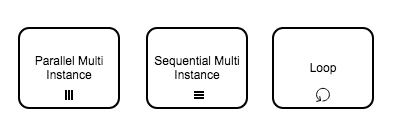
\includegraphics[scale=0.5]{../figures/chapter_combinations/BPMN_Task_Table/Multi_instance.png} \end{center}\\
\hline
A service task executes decisions in an automated way. The corresponding decision model, however, does not guarantee the automated execution. &\begin{center}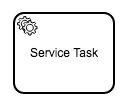
\includegraphics[scale=0.7]{../figures/chapter_combinations/BPMN_Task_Table/Service_task.png} \end{center}\\
\hline
The assignee has to execute the decision manually. &\begin{center}\includegraphics[scale=0.7]{../figures/chapter_combinations/BPMN_Task_Table/User_task.png} \end{center}\\
\hline
The Business Rule Task is defined as a placeholder according to \cite{BPMNspec} for decisional services. This is the predefined interface for DMN models. &\begin{center}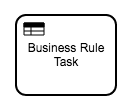
\includegraphics[scale=0.7]{../figures/chapter_combinations/BPMN_Task_Table/Business_rule_task.png} \end{center}\\
\hline
Decisions can be encoded by process script languages.  &\begin{center}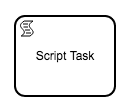
\includegraphics[scale=0.7]{../figures/chapter_combinations/BPMN_Task_Table/Script_task.png} \end{center}\\
\hline
\end{tabular}
\caption{BPMN elements and their DMN compatibility, adopted from Table 70 in \cite{DMNspec2016}.}
\label{tab:BPMN_elements_DMN_compatibility} 
\end{table}
%
%------------------------------------------------------------------------------------------------------------------------
% FIGURE ||
%            v     
%
\begin{figure}
\centering 
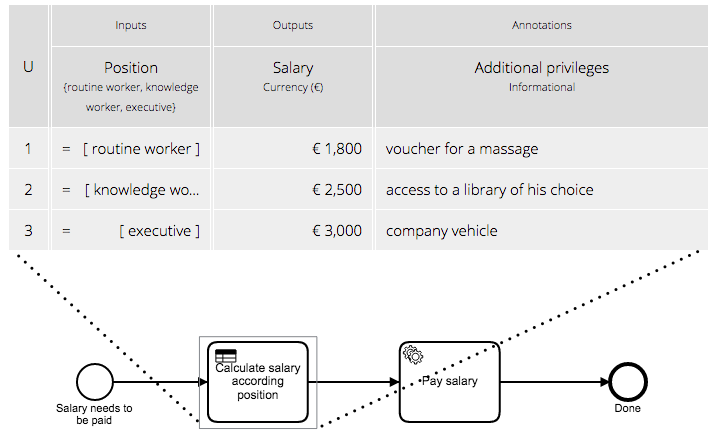
\includegraphics[width=\textwidth]{../figures/chapter_combinations/BPMN_DMN_Salary_2in1.png} 
\caption{The DMN decision logic implemented as a BPMN business rule (illustrating example).}
\label{fig:DMN_table_in_BusinessRuleTask}
\end{figure}
%
%--------------------------------------------------------------------------------------------------------------------------------------------;;;;;;;;;;;;;;;;;;;;;;;;;;;;;;;;;;;;;;;;;;;;;;;;;;;;;;;;;;;;;;;;;;;;;;;;;;;;;;;;;;;;;;;;;;;;;;;;;;;;;;;;;;;;;;;;;;;;;;;;;;;;;;;;;;;;;;;;;;;;;;;;;;;;;;;;;;;;;;;;;;;;;;;;;;;;;;;;;;;;;;;;;;;;;;;;;;;;;;;;;;;;;;;;;;;;;;;;;;;;;;;;;;;;;;;;;;;;;;;;;;;;;;;;;;;;;;;;;;;;;;;;;;;;;;;;;;;;;;;;;;;;;;;;;;;;;;;;;;;;;;;;;;;;;;;;;;;;;;;;;;;;;;;;;;;;;;;;;;;;;;;;;;;;;;;;;;;;;;;;;;;;;;;;;;;;;;;;;;;;;;;;;;;;;;;;;;;;;;;;;;;;;;;;;;;;;;;;;;;;;;;;;;;;;;;;;;;;;;;;;;;;;;;;;;;;;;;;;;;;;;;;;;;;;;;;;;;;;;;;;;;;;;;;;;;;;;;;;;;;;;;;;;;;;;;;;;;;;;;;;;;;;;;;;;;;;;;;;;;;;;;;;;;;;;;;;;;;;;;;;;;;;;;;;;;;;;;;;;;;;;;;;;;;;;;;;;;;;;;;;;;;;;;;;;;;;;;;;;;;;;;;;;;;;;;;;;;;;;;;;;;;;;;;;;;;;;;;;;;;;;;;;;;;;;;;;;;;;;;;;;;;;;;;;;;;;;;;;;;;;;;;;;;;;;;;;;;;;;;;;;;;;;;;;;;;;;;;;;;;;;;;;;;;;;;;;;;;;;;;;;;;;;;;;;;;;;;;;;;;;;;;;;;;;;;;;;;;;;;;;;;;;;;;;;;;;;;;;;;;;;;;;;;;;;;;;;;;;;;;;;;;;;;;;;;;;;;;;;;;;;;;;;;;;;;;;;;;;;;;;;;;;;;;;;;;;;;;;;;;;;;;;;;;;;;;;;;;;;;;;;;;;;;;;;;;;;;;;;;;;;;;;;;;;;;;;;;;;;;;;;;;;;;;;;;;;;;;;;;;;;;;;;;;;;;;;;;;;;;;;;;;;;;;;;;;;;;;;;;;;;;;;;;;;;;;;;;;;;;;;;;;;;;;;;;;;;;;;;;;;;;;;;;;;;;;;;;;;;;;;;;;;;;;;;;;;;;;;;;;;;;;;;;;;;;;;;;;;;;;;;;;;;;;;;;;;;;;;;;;;;;;;;;;;;;;;;;;;;;;;;;;;;;;;;;;;;;;;;;;;;;;;;;;;;;;;;;;;;;;;;;;;;;;;;;;;;;;;;;;;;;;;;;;;;;;;;;;;;;;;;;;;;;;;;;;;;;;;;;;;;;;;;;;;;;;;;;;;;;;;;;;;;;;;;;;;;;;;;;;;;;;;;;;;;;;;;;;;;;;;;;;;;;;;;;;;;;;;;;;;;;;;;;;;;;;;;;;;;;;;;;;;;;;;;;;;;;;;;;;;;;;;;;;;;;;;;;;;;;;;;;;;;;;;;;;;;;;;;;;;;;;;;;;;;;;;;;;;;;;;;;;;;;;;;;;;;;;;;;;;;;;;;;;;;;;;;;;;;;;;;;;;;;;;;;;;;;;;;;;;;;;;;;;;;;;;;;;;;;;;;;;;;;;;;;;;;;;;;;;;;;;;;;;;;;;;;;;;;;;;;;;;;;;;;;;;;;;;;;;;;;;;;;;;;;;;;;;;;;;;;;;;;;;;;;;;;;;;;;;;;;;;;;;;;;;;;;;;;;;;;;;;;;;;;;;;;;;;;;;;;;;;;;;;;;;;;;;;;;;;;;;;;;;;;;;;;;;;;;;;;;;;;;;;;;;;;;;;;;;;;;;;;;;;;;;;;;;;;;;;;;;;;;;;;;;;;;;;;;;;;;;;;;;;;;;;;;;;;;;;;;;;;;;;;;;;;;;;;;;;;;;;;;;;;;;;;;;;;;;;;;;;;;;;;;;;;;;;;;;;;;;;;;;;;;;;;;;;;;;;;;;;;;;;;;;;;;;;;;;;;;;;;;;;;;;;;;;;;;;;;;;;;;;;;;;;;;;;;;;;;;;;;;;;;;;;;;;;;;;;;;;;;;;;;;;;;;;;;;;;;;;;;;;;;;;;;;;;;;;;;;;;;;;;;;;;;;;;;;;;;;;;;;;;;;;;;;;;;;;;;;;;;;;;;;;;;;;;;;;;;;;;;;;;;;;;;;;;;;;;;;;;;;;;;;;;;;;;;;;;;;;;;;;;;;;;;;;;;;;;;;;;;;;;;;;;;;;;;;;;;;;;;;;;;;;;;;;;;;;;;;;;;;;;;;;;;;;;;;;;;;;;;;;;;;;;;;;;;;;;;;;;;;;;;;;;;;;;;;;;;;;;;;;;;;;;;;;;;;;;;;;;;;;;;;;;;;;;;;;;;;;;;;;;;;;;;;;;;;;;;;;;;;;;;;;;;;;;;;;;;;;;;;;;;;;;;;;;;;;;;;;;;;;;;;;;;;;;;;;;;;;;;;;;;;;;;;;;;;;;;;;;;;;;;;;;;;;;;;;;;;;;;;;;;;;;;;;;;;;;;;;;;;;;;;;;;;;;;;;;;;;;;;;;;;;;;;;;;;;;;;;;;;;;;;;;;;;;;;;;;;;;;;;;;;;;;;;;;;;;;;;;;;;;;;;;;;;;;;;;;;;;;;;;;;;;;;;;;;;;;;;;;;;;;;;;;;;;;;;;;;;;;;;;;;;;;;;;;;;;;;;;;;;;;;;;;;;;;;;;;;;;;;;;;;;;;;;;;;;;;;;;;;;;;;;;;;;;;;;;;;;;;;;;;;;;;;;;;;;;;;;;;;;;;;;;;;;;;;;;;;;;;;;;;;;;;;;;;;;;;;;;;;;;;;;;;;;;;;;;;;;;;;;;;;;;;;;;;;;;;;;;;;;;;;;;;;;;;;;;;;;;;;;;;;;;;;;;;;;;;;;;;;;;;;;;;;;;;;;;;;;;;;;;;;;;;;;;;;;;;;;;;;;;;;;;;;;;;;;;;;;;;;;;;;;;;;;;;;;;;;;;;;;;;;;;;;;;;;;;;;;;;;;;;;;;;;;;;;;;;;;;;;;;;;;;;;;;;;;;;;;;;;;;;;;;;;;;;;;;;;;;;;;;;;;;;;;;;;;;;;;;;;;;;;;;;;;;;;;;;;;;;;;;;;;;;;;;;;;;;;;;;;;;;;;;;;;;;;;;;;;;;;;;;;;;;;;;;;;;;;;;;;;;;;;;;;;;;;;;;;;;;;;;;;;;;;;;;;;;;;;;;;;;;;;;;;;;;;;;;;;;;;;;;;;;;;;;;;;;;;;;;;;;;;;;;;;;;;;;;;;;;;;;;;;;;;;;;;;;;;;;;;;;;;;;;;;;;;;;;;;;;;;;;;;;;;;;;;;;;;;;;;;;;;;;;;;;;;;;;;;;;;;;;;;;;;;;;;;;;;;;;;;;;;;;;;;;;;;;;;;;;;;;;;;;;;;;;;;;;;;;;;;;;;;;;;;;;;;;;;;;;;;;;;;;;;;;;;;;;;;;;;;;;;;;;;;;;;;;;;;;;;;;;;;;;;;;;;;;;;;;;;;;;;;;;;;;;;;;;;;;;;;;;;;;;;;;;;;;;;;;;;;;;;;;;;;;;;;;;;;;;;;;;;;;;;;;;;;;;;;;;;;;;;;;;;;;;;;;;;;;;;;;;;;;;;;;;;;;;;;;;;;;;;;;;;;;;;;;;;;;;;;;;;;;;;;;;;;;;;;;;;;;;;;;;;;;;;;;;;;;;;;;;;;;;;;;;;;;;;;;;;;;;;;;;;;;;;;;;;;;;;;;;;;;;;;;;;;;;;;;;;;;;;;;;;;;;;;;;;;;;;;;;;;;;;;;;;;;;;;;;;;;;;;;;;;;;;;;;;;;;;;;;;;;;;;;;;;;;;;;;;;;;;;;;;;;;;;;;;;;;;;;;;;;;;;;;;;;;;;;;;;;;;;;;;;;;;;;;;;;;;;;;;;;;;;;;;;;;;;;;;;;;;;;;;;;;;;;;;;;;;;;;;;;;;;;;;;;;;;;;;;;;;;;;;;;;;;;;;;;;;;;;;;;;;;;;;;;;;;;;;;;;;;;;;;;;;;;;;;;;;;;;;;;;;;;;;;;;;;;;;;;;;;;;;;;;;;;;;;;;;;;;;;;;;;;;;;;;;;;;;;;;;;;;;;;;;;;;;;;;;;;;;;;;;;;;;;;;;;;;;;;;;;;;;;;;;;;;;;;;;;;;;;;;;;;;;;;;;;;;;;;;;;;;;;;;;;;;;;;;;;;;;;;;;;;;;;;;;;;;;;;;;;;;;;;;;;;;;;;;;;;;;;;;;;;;;;;;;;;;;;;;;;;;;;;;;;;;;;;;;;;;;;;;;;;;;;;;;;;;;;;;;;;;;;;;;;;;;;;;;;;;;;;;;;;;;;;;;;;;;;;;;;;;;;;;;;;;;;;;;;;;;;;;;;;;;;;;;;;;;;;;;;;;;;;;;;;;;;;;;;;;;;;;;;;;;;;;;;;;;;;;;;;;;;;;;;;;;;;;;;;;;;;;;;;;;;;;;;;;;;;;;;;;;;;;;;;;;;;;;;;;;;;;;;;;;;;;;;;;;;;;;;;;;;;;;;;;;;;;;;;;;;;;;;;;;;;;;;;;;;;;;;;;;;;;;;;;;;;;;;;;;;;;;;;;;;;;;;;;;;;;;;;;;;;;;;;;;;;;;;;;;;;;;;;;;;;;;;;;;;;;;;;;;;;;;;;;;;;;;;;;;;;;;;;;;;;;;;;;;;;;;;;;;;;;;;;;;;;;;;;;;;;;;;;;;;;;;;;;;;;;;;;;;;;;;;;;;;;;;;;;;;;;;;;;;;;;;;;;;;;;;;;;;;;;;;;;;;;;;;;;;;;;;;;;;;;;;;;;;;;;;;;;;;;;;;;;;;;;;;;;;;;;;;;;;;;;;;;;;;;;;;;;;;;;;;;;;;;;;;;;;;;;;;;;;;;;;;;;;;;;;;;;;;;;;;;;;;;;;;;;;;;;;;;;;;;;;;;;;;;;;;;;;;;;;;;;;;;;;;;;;;;;;;;;;;;;;;;;;;;;;;;;;;;;;;;;;;;;;;;;;;;;;;;;;;;;;;;;;;;;;;;;;;;;;;;;;;;;;;;;;;;;;;;;;;;;;;;;;;;;;;;;;;;;;;;;;;;;;;;;;;;;;;;;;;;;;;;;;;;;;;;;;;;;;;;;;;;;;;;;;;;;;;;;;;;;;;;;;;;;;;;;;;;;;;;;;;;;;;;;;;;;;;;;;;;;;;;;;;;;;;;;;;;;;;;;;;;;;;;;;;;;;;;;;;;;;;;;;;;;;;;;;;;;;;;;;;;;;;;;;;;;;;;;;;;;;;;;;;;;;;;;;;;;;;;;;;;;;;;;;;;;;;;;;;;;;;;;;;;;;;;;;;;;;;;;;;;;;;;;;;;;;;;;;;;;;;;;;;;;;;;;;;;;;;;;;;;;;;;;;;;;;;;;;;;;;;;;;;;;;;;;;;;;;;;;;;;;;;;;;;;;;;;;;;;;;;;;;;;;;;;;;;;;;;;;;;;;;;;;;;;;;;;;;;;;;;;;;;;;;;;;;;;;;;;;;;;;;;;;;;;;;;;;;;;;;;;;;;;;;;;;;;;;;;;;;;;;;;;;;;;;;;;;;;;;;;;;;;;;;;;;;;;;;;;;;;;;;;;;;;;;;;;;;;;;;;;;;;;;;;;;;;;;;;;;;;;;;;;;;;;;;;;;;;;;;;;;;;;;;;;;;;;;;;;;;;;;;;;;;;;;;;;;;;;;;;;;;;;;;;;;;;;;;;;;;;;;;;;;;;;;;;;;;;;;;;;;;;;;;;;;;;;;;;;;;;;;;;;;;;;;;;;;;;;;;;;;;;;;;;;;;;;;;;;;;;;;;;;;;;;;;;;;;;;;;;;;;;;;;;;;;;;;;;;;;;;;;;;;;;;;;;;;;;;;;;;;;;;;;;;;;;;;;;;;;;;;;;;;;;;;;;;;;;;;;;;;;;;;;;;;;;;;;;;;;;;;;;;;;;;;;;;;;;;;;;;;;;;;;;;;;;;;;;;;;;;;;;;;;;;;;;;;;;;;;;;;;;;;;;;;;;;;;;;;;;;;;;;;;;;;;;;;;;;;;;;;;;;;;;;;;;;;;;;;;;;;;;;;;;;;;;;;;;;;;;;;;;;;;;;;;;;;;;;;;;;;;;;;;;;;;;;;;;;;;;;;;;;;;;;;;;;;;;;;;;;;;;;;;;;;;;;;;;;;;;;;;;;;;;;;;;;;;;;;;;;;;;;;;;;;;;;;;;;;;;;;;;;;;;;;;;;;;;;;;;;;;;;;;;;;;;;;;;;;;;;;;;;;;;;;;;;;;;;;;;;;;;;;;;;;;;;;;;;;;;;;;;;;;;;;;;;;;;;;;;;;;;;;;;;;;;;;;;;;;;;;;;;;;;;;;;;;;;;;;;;;;;;;;;;;;;;;;;;;;;;;;;;;;;;;;;;;;;;;;;;;;;;;;;;;;;;;;;;;;;;;;;;;;;;;;;;;;;;;;;;;;;;;;;;;;;;;;;;;;;;;;;;;;;;;;;;;;;;;;;;;;;;;;;;;;;;;;;;;;;;;;;;;;;;;;;;;;;;;;;;;;;;;;;;;;;;;;;;;;;;;;;;;;;;;;;;;;;;;;;;;;;;;;;;;;;;;;;;;;;;;;;;;;;;;;;;;;;;;;;;;;;;;;;;;;;;;;;;;;;;;;;;;;;;;;;;;;;;;;;;;;;;;;;;;;;;;;;;;;;;;;;;;;;;;;;;;;;;;;;;;;;;;;;;;;;;;;;;;;;;;;;;;;;;;;;;;;;;;;;;;;;;;;;;;;;;;;;;;;;;;;;;;;;;;;;;;;;;;;;;;;;;;;;;;;;;;;;;;;;;;;;;;;;;;;;;;;;;;;;;;;;;;;;;;;;;;;;;;;;;;;;;;;;;;;;;;;;;;;;;;;;;;;;;;;;;;;;;;;;;;;;;;;;;;;;;;;;;;;;;;;;;;;;;;;;;;;;;;;;;;;;;;;;;;;;;;;;;;;;;;;;;;;;;;;;;;;;;;;;;;;;;;;;;;;;;;;;;;;;;;;;;;;;;;;;;;;;;;;;;;;;;;;;;;;;;;;;;;;;;;;;;;;;;;;;;;;;;;;;;;;;;;;;;;;;;;;;;;;;;;;;;;;;;;;;;;;;;;;;;;;;;;;;;;;;;;;;;;;;;;;;;;;;;;;;;;;;;;;;;;;;;;;;;;;;;;;;;;;;;;;;;;;;;;;;;;;;;;;;;;;;;;;;;;;;;;;;;;;;;;;;;;;;;;;;;;;;;;;;;;;;;;;;;;;;;;;;;;;;;;;;;;;;;;;;;;;;;;;;;;;;;;;;;;;;;;;;;;;;;;;;;;;;;;;;;;;;;;;;;;;;;;;;;;;;;;;;;;;;;;;;;;;;;;;;;;;;;;;;;;;;;;;;;;;;;;;;;;;;;;;;;;;;;;;;;;;;;;;;;;;;;;;;;;;;;;;;;;;;;;;;;;;;;;;;;;;;;;;;;;;;;;;;;;;;;;;;;;;;;;;;;;;;;;;;;;;;;;;;;;;;;;;;;;;;;;;;;;;;;;;;;;;;;;;;;;;;;;;;;;;;;;;;;;;;;;;;;;;;;;;;;;;;;;;;;;;;;;;;;;;;;;;;;;;;;;;;;;;;;;;;;;;;;;;;;;;;;;;;;;;;;;;;;;;;;;;;;;;;;;;;;;;;;;;;;;;;;;;;;;;;;;;;;;;;;;;;;;;;;;;;;;;;;;;;;;;;;;;;;;;;;;;;;;;;;;;;;;;;;;;;;;;;;;;;;;;;;;;;;;;;;;;;;;;;;;;;;;;;;;;;;;;;;;;;;;;;;;;;;;;;;;;;;;;;;;;;;;;;;;;;;;;;;;;;;;;;;;;;;;;;;;;;;;;;;;;;;;;;;;;;;;;;;;;;;;;;;;;;;;;;;;;;;;;;;;;;;;;;;;;;;;;;;;;;;;;;;;;;;;;;;;;;;;;;;;;;;;;;;;;;;;;;;;;;;;;;;;;;;;;;;;;;;;;;;;;;;;;;;;;;;;;;;;;;;;;;;;;;;;;;;;;;;;;;;;;;;;;;;;;;;;;;;;;;;;;;;;;;;;;;;;;;;;;;;;;;;;;;;;;;;;;;;;;;;;;;;;;;;;;;;;;;;;;;;;;;;;;;;;;;;;;;;;;;;;;;;;;;;;;;;;;;;;;;;;;;;;;;;;;;;;;;;;;;;;;;;;;;;;;;;;;;;;;;;;;;;;;;;;;;;;;;;;;;;;;;;;;;;;;;;;;;;;;;;;;;;;;;;;;;;;;;;;;;;;;;;;;;;;;;;;;;;;;;;;;;;;;;;;;;;;;;;;;;;;;;;;;;;;;;;;;;;;;;;;;;;;;;;;;;;;;;;;;;;;;;;;;;;;;;;;;;;;;;;;;;;;;;;;;;;;;;;;;;;;;;;;;;;;;;;;;;;;;;;;;;;;;;;;;;;;;;;;;;;;;;;;;;;;;;;;;;;;;;;;;;;;;;;;;;;;;;;;;;;;;;;;;;;;;;;;;;;;;;;;;;;;;;;;;;;;;;;;;;;;;;;;;;;;;;;;;;;;;;;;;;;;;;;;;;;;;;;;;;;;;;;;;;;;;;;;;;;;;;;;;;;;;;;;;;;;;;;;;;;;;;;;;;;;;;;;;;;;;;;;;;;;;;;;;;;;;;;;;;;;;;;;;;;;;;;;;;;;;;;;;;;;;;;;;;;;;;;;;;;;;;;;;;;;;;;;;;;;;;;;;;;;;;;;;;;;;;;;;;;;;;;;;;;;;;;;;;;;;;;;;;;;;;;;;;;;;;;;;;;;;;;;;;;;;;;;;;;;;;;;;;;;;;;;;;;;;;;;;;;;;;;;;;;;;;;;;;;;;;;;;;;;;;;;;;;;;;;;;;;;;;;;;;;;;;;;;;;;;;;;;;;;;;;;;;;;;;;;;;;;;;;;;;;;;;;;;;;;;;;;;;;;;;;;;;;;;;;;;;;;;;;;;;;;;;;;;;;;;;;;;;;;;;;;;;;;;;;;;;;;;;;;;;;;;;;;;;;;;;;;;;;;;;;;;;;;;;;;;;;;;;;;;;;;;;;;;;;;;;;;;;;;;;;;;;;;;;;;;;;;;;;;;;;;;;;;;;;;;;;;;;;;;;;;;;;;;;;;;;;;;;;;;;;;;;;;;;;;;;;;;;;;;;;;;;;;;;;;;;;;;;;;;;;;;;;;;;;;;;;;;;;;;;;;;;;;;;;;;;;;;;;;;;;;;;;;;;;;;;;;;;;;;;;;;;;;;;;;;;;;;;;;;;;;;;;;;;;;;;;;;;;;;;;;;;;;;;;;;;;;;;;;;;;;;;;;;;;;;;;;;;;;;;;;;;;;;;;;;;;;;;;;;;;;;;;;;;;;;;;;;;;;;;;;;;;;;;;;;;;;;;;;;;;;;;;;;;;;;;;;;;;;;;;;;;;;;;;;;;;;;;;;;;;;;;;;;;;;;;;;;;;;;;;;;;;;;;;;;;;;;;;;;;;;;;;;;;;;;;;;;;;;;;;;;;;;;;;;;;;;;;;;;;;;;;;;;;;;;;;;;;;;;;;;;;;;;;;;;;;;;;;;;;;;;;;;;;;;;;;;;;;;;;;;;;;;;;;;;;;;;;;;;;;;;;;;;;;;;;;;;;;;;;;;;;;;;;;;;;;;;;;;;;;;;;;;;;;;;;;;;;;;;;;;;;;;;;;;;;;;;;;;;;;;;;;;;;;;;;;;;;;;;;;;;;;;;;;;;;;;;;;;;;;;;;;;;;;;;;;;;;;;;;;;;;;;;;;;;;;;;;;;;;;;;;;;;;;;;;;;;;;;;;;;;;;;;;;;;;;;;;;;;;;;;;;;;;;;;;;;;;;;;;;;;;;;;;;;;;;;;;;;;;;;;;;;;;;;;;;;;;;;;;;;;;;;;;;;;;;;;;;;;;;;;;;;;;;;;;;;;;;;;;;;;;;;;;;;;;;;;;;;;;;;;;;;;;;;;;;;;;;;;;;;;;;;;;;;;;;;;;;;;;;;;;;;;;;;;;;;;;;;;;;;;;;;;;;;;;;;;;;;;;;;;;;;;;;;;;;;;;;;;;;;;;;;;;;;;;;;;;;;;;;;;;;;;;;;;;;;;;;;;;;;;;;;;;;;;;;;;;;;;;;;;;;;;;;;;;;;;;;;;;;;;;;;;;;;;;;;;;;;;;;;;;;;;;;;;;;;;;;;;;;;;;;;;;;;;;;;;;;;;;;;;;;;;;;;;;;;;;;;;;;;;;;;;;;;;;;;;;;;;;;;;;;;;;;;;;;;;;;;;;;;;;;;;;;;;;;;;;;;;;;;;;;;;;;;;;;;;;;;;;;;;;;;;;;;;;;;;;;;;;;;;;;;;;;;;;;;;;;;;;;;;;;;;;;;;;;;;;;;;;;;;;;;;;;;;;;;;;;;;;;;;;;;;;;;;;;;;;;;;;;;;;;;;;;;;;;;;;;;;;;;;;;;;;;;;;;;;;;;;;;;;;;;;;;;;;;;;;;;;;;;;;;;;;;;;;;;;;;;;;;;;;;;;;;;;;;;;;;;;;;;;;;;;;;;;;;;;;;;;;;;;;;;;;;;;;;;;;;;;;;;;;;;;;;;;;;;;;;;;;;;;;;;;;;;;;;;;;;;;;;;;;;;;;;;;;;;;;;;;;;;;;;;;;;;;;;;;;;;;;;;;;;;;;;;;;;;;;;;;;;;;;;;;;;;;;;;;;;;;;;;;;;;;;;;;;;;;;;;;;;;;;;;;;;;;;;;;;;;;;;;;;;;;;;;;;;;;;;;;;;;;;;;;;;;;;;;;;;;;;;;;;;;;;;;;;;;;;;;;;;;;;;;;;;;;;;;;;;;;;;;;;;;;;;;;;;;;;;;;;;;;;;;;;;;;;;;;;;;;;;;;;;;;;;;;;;;;;;;;;;;;;;;;;;;;;;;;;;;;;;;;;;;;;;;;;;;;;;;;;;;;;;;;;;;;;;;;;;;;;;;;;;;;;;;;;;;;;;;;;;;;;;;;;;;;;;;;;;;;;;;;;;;;;;;;;;;;;;;;;;;;;;;;;;;;;;;;;;;;;;;;;;;;;;;;;;;;;;;;;;;;;;;;;;;;;;;;;;;;;;;;;;;;;;;;;;;;;;;;;;;;;;;;;;;;;;;;;;;;;;;;;;;;;;;;;;;;;;;;;;;;;;;;;;;;;;;;;;;;;;;;;;;;;;;;;;;;;;;;;;;;;;;;;;;;;;;;;;;;;;;;;;;;;;;;;;;;;;;;;;;;;;;;;;;;;;;;;;;;;;;;;;;;;;;;;;;;;;;;;;;;;;;;;;;;;;;;;;;;;;;;;;;;;;;;;;;;;;;;;;;;;;;;;;;;;;;;;;;;;;;;;;;;;;;;;;;;;;;;;;;;;;;;;;;;;;;;;;;;;;;;;;;;;;;;;;;;;;;;;;;;;;;;;;;;;;;;;;;;;;;;;;;;;;;;;;;;;;;;;;;;;;;;;;;;;;;;;;;;;;;;;;;;;;;;;;;;;;;;;;;;;;;;;;;;;;;;;;;;;;;;;;;;;;;;;;;;;;;;;;;;;;;;;;;;;;;;;;;;;;;;;;;;;;;;;;;;;;;;;;;;;;;;;;;;;;;;;;;;;;;;;;;;;;;;;;;;;;;;;;;;;;;;;;;;;;;;;;;;;;;;;;;;;;;;;;;;;;;;;;;;;;;;;;;;;;;;;;;;;;;;;;;;;;;;;;;;;;;;;;;;;;;;;;;;;;;;;;;;;;;;;;;;;;;;;;;;;;;;;;;;;;;;;;;;;;;;;;;;;;;;;;;;;;;;;;;;;;;;;;;;;;;;;;;;;;;;;;;;;;;;;;;;;;;;;;;;;;;;;;;;;;;;;;;;;;;;;;;;;;;;;;;;;;;;;;;;;;;;;;;;;;;;;;;;;;;;;;;;;;;;;;;;;;;;;;;;;;;;;;;;;;;;;;;;;;;;;;;;;;;;;;;;;;;;;;;;;;;;;;;;;;;;;;;;;;;;;;;;;;;;;;;;;;;;;;;;;;;;;;;;;;;;;;;;;;;;;;;;;;;;;;;;;;;;;;;;;;;;;;;;;;;;;;;;;;;;;;;;;;;;;;;;;;;;;;;;;;;;;;;;;;;;;;;;;;;;;;;;;;;;;;;;;;;;;;;;;;;;;;;;;;;;;;;;;;;;;;;;;;;;;;;;;;;;;;;;;;;;;;;;;;;;;;;;;;;;;;;;;;;;;;;;;;;;;;;;;;;;;;;;;;;;;;;;;;;;;;;;;;;;;;;;;;;;;;;;;;;;;;;;;;;;;;;;;;;;;;;;;;;;;;;;;;;;;;;;;;;;;;;;;;;;;;;;;;;;;;;;;;;;;;;;;;;;;;;;;;;;;;;;;;;;;;;;;;;;;;;;;;;;;;;;;;;;;;;;;;;;;;;;;;;;;;;;;;;;;;;;;;;;;;;;;;;;;;;;;;;;;;;;;;;;;;;;;;;;;;;;;;;;;;;;;;;;;;;;;;;;;;;;;;;;;;;;;;;;;;;;;;;;;;;;;;;;;;;;;;;;;;;;;;;;;;;;;;;;;;;;;;;;;;;;;;;;;;;;;;;;;;;;;;;;;;;;;;;;;;;;;;;;;;;;;;;;;;;;;;;;;;;;;;;;;;;;;;;;;;;;;;;;;;;;;;;;;;;;;;;;;;;;;;;;;;;;;;;;;;;;;;;;;;;;;;;;;;;;;;;;;;;;;;;;;;;;;;;;;;;;;;;;;;;;;;;;;;;;;;;;;;;;;;;;;;;;;;;;;;;;;;;;;;;;;;;;;;;;;;;;;;;;;;;;;;;;;;;;;;;;;;;;;;;;;;;;;;;;;;;;;;;;;;;;;;;;;;;;;;;;;;;;;;;;;;;;;;;;;;;;;;;;;;;;;;;;;;;;;;;;;;;;;;;;;;;;;;;;;;;;;;;;;;;;;;;;;;;;;;;;;;;;;;;;;;;;;;;;;;;;;;;;;;;;;;;;;;;;;;;;;;;;;;;;;;;;;;;;;;;;;;;;;;;;;;;;;;;;;;;;;;;;;;;;;;;;;;;;;;;;;;;;;;;;;;;;;;;;;;;;;;;;;;;;;;;;;;;;;;;;;;;;;;;;;;;;;;;;;;;;;;;;;;;;;;;;;;;;;;;;;;;;;;;;;;;;;;;;;;;;;;;;;;;;;;;;;;;;;;;;;;;;;;;;;;;;;;;;;;;;;;;;;;;;;;;;;;;;;;;;;;;;;;;;;;;;;;;;;;;;;;;;;;;;;;;;;;;;;;;;;;;;;;;;;;;;;;;;;;;;;;;;;;;;;;;;;;;;;;;;;;;;;;;;;;;;;;;;;;;;;;;;;;;;;;;;;;;;;;;;;;;;;;;;;;;;;;;;;;;;;;;;;;;;;;;;;;;;;;;;;;;;;;;;;;;;;;;;;;;;;;;;;;;;;;;;;;;;;;;;;;;;;;;;;;;;;;;;;;;;;;;;;;;;;;;;;;;;;;;;;;;;;;;;;;;;;;;;;;;;;;;;;;;;;;;;;;;;;;;;;;;;;;;;;;;;;;;;;;;;;;;;;;;;;;;;;;;;;;;;;;;;;;;;;;;;;;;;;;;;;;;;;;;;;;;;;;;;;;;;;;;;;;;;;;;;;;;;;;;;;;;;;;;;;;;;;;;;;;;;;;;;;;;;;;;;;;;;;;;;;;;;;;;;;;;;;;;;;;;;;;;;;;;;;;;;;;;;;;;;;;;;;;;;;;;;;;;;;;;;;;;;;;;;;;;;;;;;;;;;;;;;;;;;;;;;;;;;;;;;;;;;;;;;;;;;;;;;;;;;;;;;;;;;;;;;;;;;;;;;;;;;;;;;;;;;;;;;;;;;;;;;;;;;;;;;;;;;;;;;;;;;;;;;;;;;;;;;;;;;;;;;;;;;;;;;;;;;;;;;;;;;;;;;;;;;;;;;;;;;;;;;;;;;;;;;;;;;;;;;;;;;;;;;;;;;;;;;;;;;;;;;;;;;;;;;;;;;;;;;;;;;;;;;;;;;;;;;;;;;;;;;;;;;;;;;;;;;;;;;;;;;;;;;;;;;;;;;;;;;;;;;;;;;;;;;;;;;;;;;;;;;;;;;;;;;;;;;;;;;;;;;;;;;;;;;;;;;;;;;;;;;;;;;;;;;;;;;;;;;;;;;;;;;;;;;;;;;;;;;;;;;;;;;;;;;;;;;;;;;;;;;;;;;;;;;;;;;;;;;;;;;;;;;;;;;;;;;;;;;;;;;;;;;;;;;;;;;;;;;;;;;;;;;;;;;;;;;;;;;;;;;;;;;;;;;;;;;;;;;;;;;;;;;;;;;;;;;;;;;;;;;;;;;;;;;;;;;;;;;;;;;;;;;;;;;;;;;;;;;;;;;;;;;;;;;;;;;;;;;;;;;;;;;;;;;;;;;;;;;;;;;;;;;;;;;;;;;;;;;;;;;;;;;;;;;;;;;;;;;;;;;;;;;;;;;;;;;;;;;;;;;;;;;;;;;;;;;;;;;;;;;;;;;;;;;;;;;;;;;;;;;;;;;;;;;;;;;;;;;;;;;;;;;;;;;;;;;;;;;;;;;;;;;;;;;;;;;;;;;;;;;;;;;;;;;;;;;;;;;;;;;;;;;;;;;;;;;;;;;;;;;;;;;;;;;;;;;;;;;;;;;;;;;;;;;;;;;;;;;;;;;;;;;;;;;;;;;;;;;;;;;;;;;;;;;;;;;;;;;;;;;;;;;;;;;;;;;;;;;;;;;;;;;;;;;;;;;;;;;;;;;;;;;;;;;;;;;;;;;;;;;;;;;;;;;;;;;;;;;;;;;;;;;;;;;;;;;;;;;;;;;;;;;;;;;;;;;;;;;;;;;;;;;;;;;;;;;;;;;;;;;;;;;;;;;;;;;;;;;;;;;;;;;;;;;;;;;;;;;;;;;;;;;;;;;;;;;;;;;;;;;;;;;;;;;;;;;;;;;;;;;;;;;;;;;;;;;;;;;;;;;;;;;;;;;;;;;;;;;;;;;;;;;;;;;;;;;;;;;;;;;;;;;;;;;;;;;;;;;;;;;;;;;;;;;;;;;;;;;;;;;;;;;;;;;;;;;;;;;;;;;;;;;;;;;;;;;;;;;;;;;;;;;;;;;;;;;;;;;;;;;;;;;;;;;;;;;;;;;;;;;;;;;;;;;;;;;;;;;;;;;;;;;;;;;;;;;;;;;;;;;;;;;;;;;;;;;;;;;;;;;;;;;;;;;;;;;;;;;;;;;;;;;;;;;;;;;;;;;;;;;;;;;;;;;;;;;;;;;;;;;;;;;;;;;;;;;;;;;;;;;;;;;;;;;;;;;;;;;;;;;;;;;;;;;;;;;;;;;;;;;;;;;;;;;;;;;;;;;;;;;;;;;;;;;;;;;;;;;;;;;;;;;;;;;;;;;;;;;;;;;;;;;;;;;;;;;;;;;;;;;;;;;;;;;;;;;;;;;;;;;;;;;;;;;;;;;;;;;;;;;;;;;;;;;;;;;;;;;;;;;;;;;;;;;;;;;;;;;;;;;;;;;;;;;;;;;;;;;;;;;;;;;;;;;;;;;;;;;;;;;;;;;;;;;;;;;;;;;;;;;;;;;;;;;;;;;;;;;;;;;;;;;;;;;;;;;;;;;;;;;;;;;;;;;;;;;;;;;;;;;;;;;;;;;;;;;;;;;;;;;;;;;;;;;;;;;;;;;;;;;;;;;;;;;;;;;;;;;;;;;;;;;;;;;;;;;;;;;;;;;;;;;;;;;;;;;;;;;;;;;;;;;;;;;;;;;;;;;;;;;;;;;;;;;;;;;;;;;;;;;;;;;;;;;;;;;;;;;;;;;;;;;;;;;;;;;;;;;;;;;;;;;;;;;;;;;;;;;;;;;;;;;;;;;;;;;;;;;;;;;;;;;;;;;;;;;;;;;;;;;;;;;;;;;;;;;;;;;;;;;;;;;;;;;;;;;;;;;;;;;;;;;;;;;;;;;;;;;;;;;;;;;;;;;;;;;;;;;;;;;;;;;;;;;;;;;;;;;;;;;;;;;;;;;;;;;;;;;;;;;;;;;;;;;;;;;;;;;;;;;;;;;;;;;;;;;;;;;;;;;;;;;;;;;;;;;;;;;;;;;;;;;;;;;;;;;;;;;;;;;;;;;;;;;;;;;;;;;;;;;;;;;;;;;;;;;;;;;;;;;;;;;;;;;;;;;;;;;;;;;;;;;;;;;;;;;;;;;;;;;;;;;;;;;;;;;;;;;;;;;;;;;;;;;;;;;;;;;;;;;;;;;;;;;;;;;;;;;;;;;;;;;;;;;;;;;;;;;;;;;;;;;;;;;;;;;;;;;;;;;;;;;;;;;;;;;;;;;;;;;;;;;;;;;;;;;;;;;;;;;;;;;;;;;;;;;;;;;;;;;;;;;;;;;;;;;;;;;;;;;;;;;;;;;;;;;;;;;;;;;;;;;;;;;;;;;;;;;;;;;;;;;;;;;;;;;;;;;;;;;;;;;;;;;;;;;;;;;;;;;;;;;;;;;;;;;;;;;;;;;;;;;;;;;;;;;;;;;;;;;;;;;;;;;;;;;;;;;;;;;;;;;;;;;;;;;;;;;;;;;;;;;;;;;;;;;;;;;;;;;;;;;;;;;;;;;;;;;;;;;;;;;;;;;;;;;;;;;;;;;;;;;;;;;;;;;;;;;;;;;;;;;;;;;;;;;;;;;;;;;;;;;;;;;;;;;;;;;;;;;;;;;;;;;;;;;;;;;;;;;;;;;;;;;;;;;;;;;;;;;;;;;;;;;;;;;;;;;;;;;;;;;;;;;;;;;;;;;;;;;;;;;;;;;;;;;;;;;;;;;;;;;;;;;;;;;;;;;;;;;;;;;;;;;;;;;;;;;;;;;;;;;;;;;;;;;;;;;;;;;;;;;;;;;;;;;;;;;;;;;;;;;;;;;;;;;;;;;;;;;;;;;;;;;;;;;;;;;;;;;;;;;;;;;;;;;;;;;;;;;;;;;;;;;;;;;;;;;;;;;;;;;;;;;;;;;;;;;;;;;;;;;;;;;;;;;;;;;;;;;;;;;;;;;
%
%

\section{Combining CMMN with DMN}
In the previous section, we examined the compatibility with DMN and BPMN, coming concluding that BPMN is able to integrate different notations. The DMN notation, on the other hand, has no ability to integrate other models, apart from providing a reference by an \ac{URI}. \\
The URI helps to identify and locate the documents or processes referenced by the Knowledge Source element. \enlargethispage{1\baselineskip}Thus, this is not an integration, but a documentation where to find the right document to acquire knowledge about the decision-making \cite{DMNspec2016}. \\
In the preceding section about the integration of CMMN and BPMN we found out, that the integration of Business Processes, particularly BPMN processes, is possible in CMMN. Business processes, especially \ac{BPMN} or \ac{WSBPEL}, are imperative modeling languages. They focus on two concepts according to \cite{FahlandLuebkeMendlingEtAl2009}: "The continuous changes of the process' objects" and the "[...] distinct actions, events, and changes of the process and how these can possibly succeed each other." A DMN decision can behave similar, but additionally has declarative parts. This leads to the question whether it is possible or useful to integrate DMN into CMMN. \\
The compatibility is the first and foremost question that needs to be answered. CMMN offers two ways to link external models with the process: \textit{Case Tasks} and \textit{Process Tasks}. A Case Task can only establish a link to another Case. A process task can link to business processes. DMN is per se not defined as a business process modeling language. It serves as a complementary modeling language to map decisions and their requirements. In general, this works more in a declarative way than in a imperative. Thus, the CMMN standard does not intend to link DMN with CMMN. \\ %KOMMENTIERTER TEXT STAND HIER NACH 
This holds for the current version of the standard. At the time this thesis was in conducted, the latest version available was CMMN v1.0. However, the OMG published a beta version of the upcoming CMMN specification: version 1.1 \cite{CMMNbeta}. In this version, a dedicated interface to DMN models is added (see Figure \ref{fig:CMMN_with_Decision_task}). A \textit{Decision Task} with a \textit{decisionRef : Decision} attribute referencing the DMN model establishes the missing link. The attribute \textit{implementationType : URI} specifically states the compatibility with the DMN notation. Similar to the \textit{Business Rule Task} in BPMN, there are input and output parameters of type \textit{DecisionParameter} and another one, \textit{externalRef : QName}, defining the exact decision to be used \cite{CMMNbeta}. 
Conclusively, the OMG intends to support automated and data-centric decision-making in CMMN with the upcoming version of the CMMN specification.   \\

%------------------------------------------------------------------------
\begin{figure}
\centering
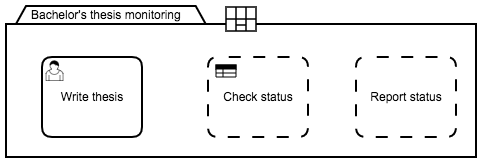
\includegraphics[width=0.8\textwidth]{../figures/chapter_combinations/CMMN_thesis_decision_task.png} 
\caption{CMMN case with a decision task linking to a DMN decision table.}
\label{fig:CMMN_with_Decision_task}
\end{figure}
%-------------------------------------------------------------------------

Figure \ref{fig:CMMN_with_Decision_task} shows a simple case with a discretionary decision task modeled. The scenario deals with a student who has to write his bachelor's thesis (see Human Task) and is monitored by his supervisor. The decision task incorporates the decision logic and links to a DMN table.\\
 When the case worker, needs to report the thesis' status to his supervisor, he checks the decision table that aggregates the information and outputs the status. In this example, the worker simply enters the amount of written pages and a comment, for instance \textit{on track} or \textit{far behind}, is presented. Afterwards, the result is sent to the supervisor.\\ 
This brief example demonstrated an automated decision making in an environment, where the focus is on human behavior and reaction. As DMN serves not only as a \textit{decision-making} notation, but also as a possibility to process data and generate an output in a fast and flexible way, it helps knowledge workers to react to data-intensive tasks and to plan following discretionary steps. 

\section{Summary}
The preceding sections demonstrated possible combinations of BPMN, DMN and CMMN. As the oldest modeling notation, BPMN has designated interfaces to call processes modeled in different notations and is able to integrate both, DMN and CMMN. CMMN, however, lacks the interface to a DMN model, which will be fixed with the next release of the specification. DMN, however, has no possibility to integrate any processes apart from DMN ones. This underlines again the complementary character of the DMN notation. 

%At this point we can conclude: there is nothing mentioned in the specification to link DMN processes. Examining the Signavio modeler (version 10.5.0, September 2016), it apparently is possible to link DMN models with a process with task. The camunda modeler (version 1.3.0, September 2016) is also able make a reference to a DMN process. However, there are inconsistencies. Listing \ref{xml:signavio} represents a snippet of XML code that is generated with signavio modeler. The snippet focuses on the process task with the linked DMN model. However, there is no reference to the linked model, which is either due to the current beta status or an incompatibility. Listing \ref{xml:camunda} shows another XML file of a CMMN model with the exact same process task and a DMN model linked. This time modeled in with the Camunda modeler. 
%
%\begin{lstlisting}[caption=XML file of a process task modeled with signavio modeler, label=xml:signavio]
%	<rdf:Description rdf:about="#sid-0083FC24-78CC-4C77-B527-5BC8B8956439">
%		<type xmlns="http://oryx-editor.org/">ProcessTask</type>
%		<bounds xmlns="http://oryx-editor.org/">261.4288403563878,97.08155333081379,
%		162.28652106916334,17.24465999244137</bounds>
%		<discretionary xmlns="http://oryx-editor.org/">false</discretionary>
%		<entry xmlns="http://oryx-editor.org/">/model/5a1ebf9abcce4bbdbd04a3b9d1652d6a</entry>
%		<bgcolor xmlns="http://oryx-editor.org/">#FFFFCC</bgcolor>
%		<name xmlns="http://oryx-editor.org/">test
%		</name>
%		<description xmlns="http://oryx-editor.org/"/>
%		<type xmlns="http://oryx-editor.org/">http://signavio.com/stencilsets/cmmn-1.0#Task</type>
%		<repetition xmlns="http://oryx-editor.org/">false</repetition>
%		<manualactivation xmlns="http://oryx-editor.org/">false</manualactivation>
%		<required xmlns="http://oryx-editor.org/">false</required>
%		<bordercolor xmlns="http://oryx-editor.org/">#000000</bordercolor>
%		<docker xmlns="http://oryx-editor.org/"> # </docker>
%		<parent xmlns="http://raziel.org/" rdf:resource="#sid-F6DDC76E-A454-4C2F-A7D1-4121A78A527F"/>
%	</rdf:Description>
%\end{lstlisting} 
%
%\begin{lstlisting}[caption=A Process Task modeled with camunda modeler, label=xml:camunda]
%  <cmmn:case id="Case_1">
%    <cmmn:casePlanModel id="CasePlanModel_1" name="A CasePlanModel">
%      <cmmn:planItem id="PlanItem_1" definitionRef="ProcessTask_1nzv0h6" />
%      <cmmn:processTask id="ProcessTask_1nzv0h6" name="TASK" processRef="DMN_MODEL.dmn" /> |\label{line:processRef}|
%    </cmmn:casePlanModel>
%  </cmmn:case>
%\end{lstlisting}
%
%Here, in line \ref{line:processRef} of Listing \ref{xml:camunda}, the reference to the DMN model is documented, whereas Listing \ref{xml:signavio} does not provide any reference to the according attribute, although the process is visually linked in the modeler. Unfortunately, it wasn't possible to execute neither the camunda version nor the signavio one. The latter is still in beta phase and the former one cannot be executed without any licensing. We asked for an academic license but could not acquire one. \\
%Reviewing the results, integrating DMN in CMMN is not namely intended, but it seems possible. The Camunda example showed a reference that could be set to a DMN model, which was also possible with the Signavio modeler. However, the Signavio XML file did not show the \textit{processRef} attribute which, in fact, is the link to external processes. \\
%Integrating CMMN in DMN, on the other hand, is impossible as DMN has not interface to external processes such as BPMN Call Activities or CMMN Process Tasks. 


%
%% ---------------------------------------------------------------------------
%%
%% Fully Automated Calibration for Ultrasound
%%
%%% ---------------------------------------------------------------------------
%\part[Fully Automated Calibration for Ultrasound]{Fully Automated Calibration for Ultrasound}
%\label{part:fullyAutomatedCalibration}
%\input{chapters/FullyAutomatedCalibrationOverview} 
%\input{chapters/MethodsAndImplementation}
%\input{chapters/SpheresPhantom} 
%\input{chapters/ModulatedCirclesPhantom} 

%% ---------------------------------------------------------------------------
%%
%% Results and Conclusion
%%
%% ---------------------------------------------------------------------------
%\part[Results and Conclusion]{Results and Conclusion}
%\label{part:resultsAndConclusion}
%\input{chapters/Experiments} 
%\input{chapters/Simulations} 
%\chapter{Conclusion and future work}
\label{conclusion}
\section{The big picture}
We started this thesis with three research questions and the objective to provide a methodology to distinguish between three modeling notations and combine them in a super-model. In Chapter \ref{chapter:indicators}, a set of characteristics was formed to describe and identify processes. Starting with BPMN, we achieved to define matching processes capturing \textit{routine} work with \textit{predictable} output, ultimately resulting in as much automation as possible. In contrast, CMMN is appropriate for the opposite type of work: \textit{agile} with \textit{emerging} tasks from circumstances that can be \textit{partly automated} as well as \textit{partly predefined}. The main difference between BPMN and CMMN is the focus on workflow execution (BPMN) and supporting knowledge workers in their daily, mostly manual, business (CMMN). DMN, on the other side, is a convenient tool to cope with data intensive processes. The reason why it is called \textit{Decision} Model and Notation can be derived from the data-centric aspect. Taken into account that a preceding process documentation is comprised of a spreadsheet, eventually this spreadsheet should result in a certain output, aiding in a decision-making process. DMN is a tool that aggregates data and results in a decision. It complements data- or decision-intensive processes. However, we saw in the Chapter \ref{chapter:case_study} that data-intensive processes cannot always be complemented with DMN or even completely modeled in this notation. The eKulturPortal is a data driven application. Its first milestone is comprised of features dealing with the creation and administration of database objects such as companies, venues and users. In this case, the indicators did not recommend DMN to handle these data processes, since the type of data did not match with DMN tables. An overview of all the indicators defined in Chapter \ref{chapter:indicators} can be found in Table \ref{tab:indicators}. \\
 
% Please add the following required packages to your document preamble:
% \usepackage{booktabs}
% \usepackage{graphicx}
% \usepackage[normalem]{ulem}
% \useunder{\uline}{\ul}{}
\begin{table}[h!]
\centering
\resizebox{\textwidth}{!}{%
\begin{tabular}{@{}lllll@{}}
\toprule
Categories                   & Weighting & BPMN Indicators                                 & CMMN Indicators                                                                                & DMN Indicators                                                                                      \\ \midrule
Documentation style          & 1         & Directives                                      & \begin{tabular}[c]{@{}l@{}}Descriptions of best practices\\ and recommendations\end{tabular}   & Spreadsheets                                                                                        \\
Preceding process map        & 1         & Flowchart                                       & Cluster                                                                                        & Decision trees                                                                                      \\
Characteristics of work      & 2         & routine, predictable, automatable               & \begin{tabular}[c]{@{}l@{}}Agile, emerging, \\ partly automatable\end{tabular}                 & \begin{tabular}[c]{@{}l@{}}decision-intensive, data handling,\\ decison-making\end{tabular}         \\
Characteristics of process   & 2         & rigid, predefined, workflow-centric             & \begin{tabular}[c]{@{}l@{}}adaptive, partly predefined, \\ knowledge-centric\end{tabular}      & \begin{tabular}[c]{@{}l@{}}data-centric, data processing,\\ complementary\end{tabular}              \\
Characteristics of decisions & 2         & Simple (either / or)                            & Stateful (transition form one to another state)                                                & Complex                                                                                             \\
Control flow                 & 1         & Definite control flow, required                 & Indefinite control flow, optional                                                              & Dependencies, required                                                                              \\
Intervention at run-time     & 1         & No                                              & Yes                                                                                            & Yes                                                                                                 \\
Objective                    & 2         & Automated workflow execution                    & Support manual work                                                                            & Automated data processing                                                                           \\
Type of process              & 2         & Business process                                & Case                                                                                           & Decisions                                                                                           \\
Typical application          & 1         & Billing process, Accounting, Assembly-line work & \begin{tabular}[c]{@{}l@{}}Reviews, Medical attendance,\\ Managing and organising\end{tabular} & \begin{tabular}[c]{@{}l@{}}Calculation of discount rates, salary,\\ choosing assignees\end{tabular} \\ \midrule
Points per Indicator        & \multicolumn{4}{c}{15}                                                                                                                                                                                                                                             \\ \bottomrule
\end{tabular}%
}
\caption{An overview of the indicators defined in Chapter \ref{chapter:indicators}.}
\label{tab:indicators}
\end{table}
After the definition of indicators, the combination aspect was examined in Chapter \ref{chapter:combination}. Each notation's ability to link different notations within the model was presented. We found out, that DMN has no designated interface to any of the two modeling notations, whereas BPMN and CMMN have interfaces to link with any of the three notations. \enlargethispage{1\baselineskip}\newpage BPMN features a \textit{Call Activity} and a \textit{Business Rule Task}, both referencing either different BPMN or CMMN processes or - in terms of a \textit{Business Rule Task} - referencing to a DMN table. CMMN features designated \textit{Business Process Tasks} and \textit{Case Tasks}, as well as \textit{Decision Tasks} that reference to the according processes, ultimately supporting the case worker with automated task execution. As we saw again in this chapter, DMN is a complementary notation without a practical use case for a standalone model. \\
With these two chapters in mind, Chapter \ref{chapter:case_study} showed practical applications of the indicators and how to combine models eventually. A key process, the \textit{Company audit}, was dissected in a bottom-up approach with a top-down view, as \cite{Verner2004} recommended and endorsed by different best practices. Starting with a process map, the process documentation has lead us through the discovery process creating sub-processes according to the \textit{Separation of Concerns} paradigm. Each process captures a logical unit, making it easier and clearer to model processes with a broad variety of deliberations. To orchestrate all the sub-processes, a super-process was created with the ability to call each logical unit upon request. As the \textit{Company Audit} process features \textit{agile} characteristics and the objective to \textit{support manual work}, the recommendation for this super-model was CMMN. The conclusion shows that the mentioned combinations allow modeling all references with their designated interfaces along with CMMN's functions to report states and to listen to user events, such as an abortion of the case execution. Furthermore, some smaller processes were presented that were modeled in BPMN due to a preceding recommendation. \newpage
At this point, we can answer the three research questions from the very beginning of this thesis. The first question deals with the DMN notation and its ability to model decisions and replacing gateway modeling in BPMN. In Chapter \ref{chapter:combination} we found a way to provide a replacement of BPMN gateways and even more elements, such as finding the right assignee for a task or listening to events. DMN serves as a complementary notation, supporting BPMN by separating the concern of data handling from larger processes while making them clearer and easier to understand. The process execution might also feature a performance increase, which could be part of future work. \\
The second question deals with CMMN and the usage of cases in a software project. During the investigation of the \textit{Company Audit} process, we applied the indicators on the super-process and some sub-processes leading to several CMMN recommendations. All of the CMMN processes originate from a software development project and will be implemented in a middleware. This middleware serves as an orchestration for the portal and connects the frontend with the database layer. The implemented process consequently orchestrates the interaction between database, frontend and other systems like access rights management.\\
CMMN is a suitable way to support a system when it comes to human intervention. The auditor, for instance, is a worker that interacts with the system in a semi-automated way, because he handles the necessary checks to prove a company's authenticity. Furthermore, there will be use cases where the user, instead of a machine, is in the center of action. These processes can conveniently be modeled in CMMN, connecting automated tasks with manual ones and create a unique user experience based on partly predefined processes.\\
The last research question deals with the combination of the notations and beneficial aspects such as improved readability and information flow. Concerning the latter, this thesis could not investigate the implementation of processes and corresponding improvements about performance and information flow. Since the eKultur project still is in the design phase, nothing has been implemented while this thesis was written. None of the processes have been executed once, neither has the middleware been set up during the investigation of the processes. All mentioned processes have been modeled initially during this thesis, resulting in a lack of comparable objects, particularly process models, and data for instance cycle times or information congestion. However, the combination of models itself was investigated in detail as well as the aspect of improved readability. Especially the latter aspect can be approved by Chapter \ref{chapter:combination}, as long as the \textit{Separation of concerns} paradigm is being followed by the process analysts.\newpage It is inherent to encapsulate a single logical unit into a sub-process and orchestrating the whole set of sub-processes with a super-process. This achieves improved readability and simplifies the implementation tasks for developers. Due to smaller logical units, developers are able to create classes featuring a high cohesion and loose coupling. These classes are also characterized by improved readability and encapsulating a single logical unit. Ideally, developers can derive the code to be implemented from a complete process model with all the attributes and references set during the design phase. The combination of process models can help to improve the interface design in a technical perspective, as well as aiding the frontend engineers to decide when a user is intended to do more manual work or has to reply on question the system presents him. 

\section{Downsides of this thesis}
The major part of this thesis deals with the creation of a methodology to identify a suitable modeling language for a discovered process. Chapter \ref{chapter:indicators} and \ref{chapter:combination} carried out this intention by reviewing literature and aggregating information about the modeling notations. Consequently, the research questions could be answered. \\
However, Chapter \ref{chapter:case_study} was intended to prove the indicators, which could only be achieved to a certain extent. As part of the eKultur project and author of this thesis, a dual role was created that has lead a comparison problem. As a consequence, there is no comparable material that can be used to validate an improvement by applying the indicators to the models and re-modeling them. For this thesis, models created by different analysts should have been used to increase the provability of the methodology. \\
Another aspect is the lack of statistical data. The scope of this thesis was not to do a statistical evaluation resulting in a set of data that could be used for a proof of concept. Neither was the scope to acquire processes from different companies using them for the practical application. However, both could be part of future work that deals with a comparison.
Eventually, the practical application part of Chapter \ref{chapter:case_study} resulted in a show case on how to apply the indicators and the combination on processes along with the usage of the decision engine for the recommendation. As the title states, this thesis functions as a \textit{Guideline to combine and differentiate between BPMN, CMMN and DMN}, which was realized in the preceding chapters. The application part showed that the indicators are working for process discovery products, for instance process maps and documentation. \newpage Since eKultur uses manual process discovery, automated process discovery could not be tested. This might also be part of future work. \\
Conclusively, we were able to show a working product for processes that were manually discovered, but could not prove the concept on a larger scale. 

\section{Future work}
As stated in the section above, the large scale proof could not be achieved. Neither could the indicators be applied on results of automated process discovery. Future work could deal with a statistical evaluation of the 
 application, as well as include results from automated process discovery. Another aspect is the comparison between models that have been created without the indicators and ones implementing the recommendation system. This could measure the robustness of the concept. \\
Furthermore, the guideline in general could be tested empirically. People without knowledge about process modeling could use the guideline to learn about the three different modeling notations and be advised to create a process model from a given process documentation. Afterwards, the effectiveness of the guideline could be evaluated. Business analysts could be asked to use the guideline and give their feedback about the concept and how they would characterize certain aspects of the notations and the processes they capture. This could improve the indicators and the recommendation system. Also, the weighting seen in Table \ref{tab:indicators} is a value that has been set according to the importance of certain aspects. Future work could check the weighting and adjust it according to statistical evaluation. \\ 


% ---------------------------------------------------------------------------
%
% Appendix
%
% ---------------------------------------------------------------------------

\part*{Appendix}
\addcontentsline{toc}{part}{Appendix}

\appendix %---------------------------------------

%\input{chapters/validationDetailed}

		
		
		% ---------------------------------------------------------------------------
		%
		% Appendix
		%
		% ---------------------------------------------------------------------------
		%\newpage
%		\part*{Appendix}
%		\addcontentsline{toc}{part}{Appendix}
%		\appendix %---------------------------------------
%		\begin{appendices}
%		\input{chapters/oneAppendix}
%		\end{appendices}
%		\appendix
		\renewcommand\thechapter{}
%		\renewcommand\thesection{\arabic{section}}
		\renewcommand\thesection{}
%		\input{chapters/oneAppendix}

	\clearemptydoublepage		
	\phantomsection
	\addcontentsline{toc}{chapter}{\listfigurename}
	\listoffigures 
	
    \clearemptydoublepage
	\bibliography{bibliography/literature}
	
	
 
\end{document}

